%\documentclass[11pt,a4paper,twoside]{tesis}
% SI NO PENSAS IMPRIMIRLO EN FORMATO LIBRO PODES USAR
%\documentclass[11pt,a4paper]{tesis}
\documentclass[a4paper,12pt,single-sided]{book}

\usepackage{graphicx}
\usepackage[utf8]{inputenc}
\usepackage[spanish]{babel}
\usepackage[left=3cm,right=3cm,bottom=3.5cm,top=3.5cm]{geometry}
\usepackage{sidecap} 
\usepackage{color}
\usepackage{listings}
\usepackage{float}
\usepackage{longtable}
\usepackage[spanish]{babel}

\usepackage{pgfplots}
\pgfplotsset{width=15cm, height=8cm}

\graphicspath{ {Images/} }

\setlength{\parindent}{1em}
\setlength{\parskip}{4pt}

\begin{document}

%%%% CARATULA
% Comentar y descomentar según corresponda
%\def\titulo{Licenciada }
\def\titulo{Licenciado }

\def\autor{Fernando Bugni}
\def\tituloTesis{Recolección online de grabaciones para el estudio de las variantes argentinas del español}
\def\runtitulo{Recolección online de grabaciones para el estudio de las variantes argentinas del español}
\def\runtitle{Star Wars: Rebellion and Empire}
\def\director{Agustín Gravano}
\def\codirector{Miguel Martínez Soler}
\def\lugar{Buenos Aires, 2014}
\newcommand{\HRule}{\rule{\linewidth}{0.2mm}}
%
\thispagestyle{empty}

\begin{center}\leavevmode

\vspace{-2cm}

\begin{tabular}{l}

\includegraphics[width=2.6cm]{logofcen.pdf}
\end{tabular}


{\large \sc Universidad de Buenos Aires

Facultad de Ciencias Exactas y Naturales

Departamento de Computaci\'on}

\vspace{6.0cm}

%\vspace{3.0cm}
%{
%\Large \color{red}
%\begin{tabular}{|p{2cm}cp{2cm}|}
%\hline
%& Pre-Final Version: \today &\\
%\hline
%\end{tabular}
%}
%\vspace{2.5cm}

{\huge\bf \tituloTesis}

\vspace{2cm}

{\large Tesis presentada para optar al t\'{\i}tulo de\\
\titulo en Ciencias de la Computaci\'on}

\vspace{2cm}

{\Large \autor}

\end{center}

\vfill

{\large

{Director: \director}

\vspace{.2cm}

{Codirector: \codirector}

\vspace{.2cm}

\lugar
}

\newpage\thispagestyle{empty}


%%%% ABSTRACTS, AGRADECIMIENTOS Y DEDICATORIA
\frontmatter
\pagestyle{empty}
%\begin{center}
%\large \bf \runtitulo
%\end{center}
%\vspace{1cm}
\chapter*{\runtitulo}

\noindent 

El uso de la lengua siempre ha caracterizado a las personas que la utilizan. La forma en como nos comunicamos no sólo posee la información del mensaje a trasmitir, sino que también posee características del hablante. Estas características pueden describir al hablante de distintas formas. Algunas de ellas pueden ser: su cultura, su economía, su región entre otras. 

Particularmente en Argentina no es la excepción. Nuestro país posee una fuerte componente dialéctica en su habla. Esto quiere decir que podemos saber de que lugar proviene el hablante analizando su tonada. Hay varias regiones definidas a través del país. En este trabajo nos enfocaremos en distinguir diferencias entre la región de Córdoba y Buenos Aires. Realizaremos un experimento donde compararemos el habla de cada grupo. Utilizando estos datos analizaremos efectivamente cuales son las características mas predominantes y como repercute esas diferencias en el habla. Por último, mostraremos distintos clasificadores para determinar de que grupo proviene una grabación, analizaremos las atributos mas importantes y testearemos la solución propuesta. 

\bigskip


%\cleardoublepage
%%\begin{center}
%\large \bf \runtitle
%\end{center}
%\vspace{1cm}
\chapter*{\runtitle}

\noindent In a galaxy far, far away, a psychopathic emperor and his most trusted servant -- a former Jedi Knight known as Darth Vader -- are ruling a universe with fear. They have built a horrifying weapon known as the Death Star, a giant battle station capable of annihilating a world in less than a second. When the Death Star's master plans are captured by the fledgling Rebel Alliance, Vader starts a pursuit of the ship carrying them. A young dissident Senator, Leia Organa, is aboard the ship \& puts the plans into a maintenance robot named R2-D2. Although she is captured, the Death Star plans cannot be found, as R2 \& his companion, a tall robot named C-3PO, have escaped to the desert world of Tatooine below. Through a series of mishaps, the robots end up in the hands of a farm boy named Luke Skywalker, who lives with his Uncle Owen \& Aunt Beru. Owen \& Beru are viciously murdered by the Empire's stormtroopers who are trying to recover the plans, and Luke \& the robots meet with former Jedi Knight Obi-Wan Kenobi to try to return the plans to Leia Organa's home, Alderaan. After contracting a pilot named Han Solo \& his Wookiee companion Chewbacca, they escape an Imperial blockade. But when they reach Alderaan's coordinates, they find it destroyed - by the Death Star. They soon find themselves caught in a tractor beam \& pulled into the Death Star. Although they rescue Leia Organa from the Death Star after a series of narrow escapes, Kenobi becomes one with the Force after being killed by his former pupil - Darth Vader. They reach the Alliance's base on Yavin's fourth moon, but the Imperials are in hot pursuit with the Death Star, and plan to annihilate the Rebel base. The Rebels must quickly find a way to eliminate the Death Star before it destroys them as it did Alderaan (aprox. 200 palabras).

\bigskip

\noindent\textbf{Keywords:} War, Rebellion, Wookie, Jedi, The Force, Empire (no menos de 5).

\cleardoublepage
\chapter*{Agradecimientos}

\noindent Lorem ipsum dolor sit amet, consectetur adipiscing elit. Fusce sapien ipsum, aliquet eget convallis at, adipiscing non odio. Donec porttitor tincidunt cursus. In tellus dui, varius sed scelerisque faucibus, sagittis non magna. Vestibulum ante ipsum primis in faucibus orci luctus et ultrices posuere cubilia Curae; Mauris et luctus justo. Class aptent taciti sociosqu ad litora torquent per conubia nostra, per inceptos himenaeos. Mauris sit amet purus massa, sed sodales justo. Mauris id mi sed orci porttitor dictum. Donec vitae mi non leo consectetur tempus vel et sapien. Curabitur enim quam, sollicitudin id iaculis id, congue euismod diam. Sed in eros nec urna lacinia porttitor ut vitae nulla. Ut mattis, erat et laoreet feugiat, lacus urna hendrerit nisi, at tincidunt dui justo at felis. Class aptent taciti sociosqu ad litora torquent per conubia nostra, per inceptos himenaeos. Ut iaculis euismod magna et consequat. Mauris eu augue in ipsum elementum dictum. Sed accumsan, velit vel vehicula dignissim, nibh tellus consequat metus, vel fringilla neque dolor in dolor. Aliquam ac justo ut lectus iaculis pharetra vitae sed turpis. Aliquam pulvinar lorem vel ipsum auctor et hendrerit nisl molestie. Donec id felis nec ante placerat vehicula. Sed lacus risus, aliquet vel facilisis eu, placerat vitae augue. % OPCIONAL: comentar si no se quiere

\cleardoublepage
\hfill \textit{A mi viejo, que me ayuda desde el cielo.}

\hfill \textit{A mi vieja, que gracias a ella soy lo que soy.} 

\hfill \textit{Y a mi hermano, que es el compañero de mi vida.}  % OPCIONAL: comentar si no se quiere

\cleardoublepage
\tableofcontents

\mainmatter
\pagestyle{headings}

%%%% ACA VA EL CONTENIDO DE LA TESIS


\chapter{Introducción}

% todo: AGREGAR FONTANELLA Y VIDAL DE BATTINI
% RESCRIBIR

El uso de la lengua siempre ha caracterizado a las personas que la utilizan. La forma en que nos comunicamos no sólo posee la información del mensaje a trasmitir, sino que también posee características del hablante. Estudiar estas características del habla nos permite conocer mejor la cultura de las personas. Nos permite identificar a los hablantes para saber el lugar donde pertenecen.

Identificar y extraer características del habla es una tarea muy difícil de realizar. No solo se debe obtener muestras muy variadas de muchos hablantes en distintas regiones, sino que también hay que prestarle importante atención a su edad, su sexo, su situación económica, etc. Realizar un estudio de estas características es muy complejo y sobre todo, costoso. Además de estudiar cada grupo se debe utilizar muchos recursos: por ejemplo, se debe utilizar soporte para grabar en buena calidad las muestras ... , varios viajes para buscar los diferentes hablantes ... , analizar cada uno de los audios de manera individual, entre otras cosas. 

\begin{figure}[h!]
	\centering
    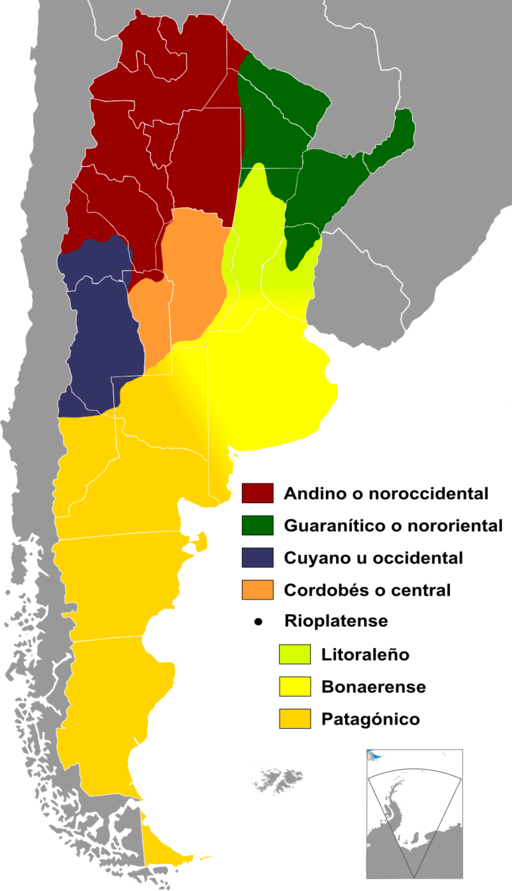
\includegraphics[width=0.5\textwidth]{Dialectos_del_idioma_espanol_en_Argentina} 
    \caption{Dialectos del idioma español en Argentina}
    \label{fig11}
\end{figure}

La objetivo de esta tesis es realizar un sistema que pueda facilitar estos problemas. Vamos a enfrentar cada uno de ellos e intentar resolverlos de forma computacional. De los problemas descriptos el principal radica en obtener cada grabación. Si los grupos se encuentran muy alejados esto puede ser muy costoso por los viajes. También estas grabaciones deben ser de calidad aceptable como para realizar el estudio en cuestión. Se podría utilizar el teléfono para algunos experimentos pero hay que tener en cuenta que este posee calidad muy baja. De hecho, se utiliza en algunos experimentos donde esta característica no es un inconveniente. 

Es por esto que se desarrolló un sistema de grabación basado en Internet como herramienta para obtener muestras. De esta forma, se puede realizar varias grabaciones sin necesidad de viajar a cada lugar. Es cierto que no todos los lugares poseen acceso a Internet y, si se realizara un experimento de estas características en lugares que no posean conexión, este sistema no sería útil. De cualquier forma, pensamos que su utilización soluciona muchos inconvenientes. Otra característica radica en que se puede manejar la calidad de la grabación. Utilizando distintas tecnologías a través de esta red se puede configurar la calidad para que sea lo más precisa posible para el experimento. El sistema desarrollado va a mejorar la forma de recolectar muestras y lo utilizamos en un experimento para corroborar las ventajas y desventajas del mismo.

El objetivo del sistema es obtener muestras de habla para su posterior análisis o utilización en sistemas de procesamiento de voz. El experimento que tomamos como caso de estudio es las diferencias en el habla entre Córdoba y Buenos Aires. El primero de estos grupos se encuentran uno en la zona central de nuestro país mientras que el segundo cerca del Río de la Plata, como se puede observar en la Figura \ref{fig11}. En la literatura existen estudios que explican estas diferencias, por ejemplo \textit{El español en la Argentina} \cite{Fontanella2000} de Beatriz Fontanella de Weinberg y \textit{Español en la Argentina} \cite{Vidal1964} de Elena Vidal de Battini. 

Fontanella de Weinberg recopila varios trabajos de colegas que analizan el español de cada región de Argentina. Cada región se describe en un capítulo distinto y entre ellas se encuentra uno para Buenos Aires y otro para Córdoba. En la descripción de estos capítulos las diferencias hacen hincapié en los sonidos más suaves y cortos de la /r/ y la /i/ y en la aspiración de la /s/. También describe el estiramiento de la sílaba anterior a la acentuada en cada palabra como distintivo del acento. Por su parte, Vidal de Battini analiza región por región el uso de los fonemas importantes. Destaca la diferencia entre las dos regiones de la /r/, /s/ y de la /ll/. También referencia a la pronunciación de la /s/.
%pagina 85 Fontanella 

Extrayendo el análisis de estos libros pude definir las reglas que describen a cada grupo. Las reglas son: 

\begin{itemize}

\item \textbf{Regla 1: Los hablantes de Córdoba estiran la sílaba anterior a la acentuada mientras los de Buenos Aires no realizan esto.} Cada palabra posee una sílaba con su acento primario. Para cumplir esta regla se debe estirar la sílaba anterior a esta. Si la sílaba acentuada es la primera de la palabra, entonces no se estira. Ejemplo: `Espectacular' posee su sílaba acentuada en `-lar'. La sílaba anterior, o sea `-cu-' se alarga solamente para hablantes de Córdoba. 

\item \textbf{Regla 2: Los hablantes de Córdoba aspiran y elisionan la /s/ al finalizar una palabra. Esto no sucede para Buenos Aires.} Para las palabras terminadas en /s/ se acorta su duración en el hablante de Córdoba. Ejemplo: `Pájaros' posee el fonema /s/ al final. Utilizando la dialéctica de Córdoba, la /s/ final sería más suave que una de Buenos Aires. 

\item \textbf{Regla 3: Para hablantes de Córdoba, la /s/ antes de la /c/ o /t/ suenan más suaves que para hablantes de Buenos Aires.} La sílaba /s/, que precede a /c/ o /t/, suena más suave en cordobeces que en porteños. Ejemplo: `Mosca' en la variante de Córdoba posee una sílaba más suave en el fonema /s/ que en Buenos Aires. 

\item \textbf{Regla 4: La `c' antes de la `t' se pronuncia con menor frecuencia para hablantes de Córdoba que para hablantes de Buenos Aires.} La sílaba /c/, que precede a /t/, no se debe pronunciar. Ejemplo: `Doctor' no debe sonar el fonema /c/.

\item \textbf{Regla 5: Para hablantes cordobeces la `y’ y `ll’ se pasa a `i’. No sucede esto para Buenos Aires.} Palabras con el fonema /y/ o /ll/ se pronuncian /j/. Ejemplo: `lluvia' se debe pronunciar utilizando el fonema /j/. 

\item \textbf{Regla 6: En hablantes cordobeces la /r/ no vibra mientras que en Buenos Aires pasa lo contrario.} Palabras con el fonema /r/ deben ser suaves y no vibrar. Ejemplo: `Espárrago' debe ser suave en comparación de Buenos Aires. 

\end{itemize}

Normalmente estas reglas se producen en el habla espontánea y raramente en habla leída. Algunas pueden agudizarse si se encuentran en lugares económicamente más vulnerables, pero en cualquier ambiente se cumple.

En el próximo capítulo describiremos el diseño del experimento. Este tiene como objetivo reconocer las diferencias planteadas con las reglas mediante la grabación de frases. Estas frases fueron grabadas tanto por hablantes de Córdoba como de Buenos Aires. También describiremos cuales frases utilizamos y el medio empleado para grabar.

\chapter{Diseño del experimento}

Utilizando los estudios de \cite{Fontanella2000} y \cite{Vidal1964} pudimos obtener las reglas definidas en el capítulo anterior. Recordemos que éstas describen la diferencia entre los dos grupos. En este capítulo proponemos realizar un experimento para extraer la información fonética de los mismos. La idea será realizar una serie de actividades donde el hablante sea grabado y que esas actividades hagan hincapié en estas diferencias descriptas. A continuación vamos a describir el experimento en más detalle.

\section{Elección de las frases}

El acento se potencia cuando se realiza habla espontánea. Utilizando este concepto intentamos que el hablante diga las frases de la forma más natural posible. Es por ello que elegimos como actividad pronunciar frases popularmente conocidas. Si el hablante conoce la frase y la utiliza con frecuencia entonces es más fácil que su pronunciación sea espontánea. Con esta idea vamos a cubrir las reglas 2 al 6. 

Recordemos que en el capítulo anterior la regla 1 nos decía que había una diferencia en la duración de la sílaba previa a la acentuada: para hablantes de Córdoba esta duración es más larga que para hablantes de Buenos Aires. La sílaba acentuada varía según que tipo de palabra se refiere. No es lo mismo utilizar una palabra aguda que una esdrújula en esta regla. Para cubrir esta regla utilizamos un esquema de frases con una estructura fija pero que varía sus palabras según su entonación. Este esquema se llama AMPER \cite{amper} y lo veremos más en detalle en la sección \ref{cap:amper}.

Entonces los esquemas van a ser: 

\begin{itemize}
  \item \textbf{Frases utilizando esquema AMPER que cubre cada tipo de acentuación:} Estas corresponden a la regla 1 que hace énfasis en la longitud de la sílaba anterior a la acentuada. Utilizamos este esquema para cubrir todo tipo de acentuación.
  \item \textbf{Frases comunes que tratan de cubrir la espontaneidad:} Estas frases van a cubrir las reglas 2 a 6. Estas tienen que ver con la duración y la pronunciación de distintos fonemas. Utilizar frases comunes favorece la espontaneidad.
\end{itemize}

A continuación vemos las reglas en sus dos conjuntos.

\subsection{Frases utilizando esquema AMPER} \label{cap:amper}

%AMPER-ARGENTINA: VARIABILIDAD RÍTMICA EN DOS CORPUS 
%Jorge A. Gurlekian LIS - Conicet y UBA jag@fmed.uba.ar 
%Reina Yanagida LIS y Universidad Municipal de Estudios Extranjeros de Kobe, Japón reinay@hotmail.co.jp 
%Mónica Noemí Trípodi LIS – UBA monica906@hotmail.com 
%Guillermo Toledo Conicet y Universidad Laval, Canadá guillermo.toledo@sympatico.ca 

Utilizamos este esquema para analizar todas las variantes posibles de la regla 1. Recordemos que esa regla nos dice que hay que estirar la sílaba anterior a la acentuada. Esta regla define comúnmente la tonada cordobeza y puede aparecer de varias formas según su acentuación. 

Para tomar este esquema nos basamos en el trabajo de variabilidad rítmica en dos corpus \cite{amper} que utilizan un esquema similar. Este trabajo estudió los acentos del español argentino utilizando un esquema de frase fija y intercambiando palabras para analizar todos sus casos. En nuestro trabajo tenemos un problema similar por ello lo tomamos como referencia.

Para el esquema AMPER se fija una estructura para la frase y se va cambiando las palabras que utiliza. El esquema AMPER utilizado en este trabajo es: 
\begin{center}
\textit{Sujeto+`` salió ’’+Adjetivo} 
\end{center}

\begin{itemize}
	\item Objeto puede ser \textit{``El canapé’’, ``El repollo’’, ``El espárrago’’}.
	\item Adjetivo puede ser \textit{``espectacular’’, ``delicioso’’, ``riquísimo’’}.
\end{itemize}

Utilizamos estas palabras ya que cubren los tres tipos de acentuación: aguda, grave y esdrújula. 

Por ejemplo: \textit{``El canapé salió delicioso’’}. Canapé tiene acento en la última sílaba, es una palabra aguda, mientras que delicioso es grave. En este ejemplo podemos analizar la sílaba anterior a la acentuada de los dos grupos estudiados, Córdoba y Buenos Aires. Armamos las combinaciones para obtener muchas variantes de dónde se encuentra el acento. De esta forma estudiamos en detalle la regla 1. Todas las combinaciones se pueden ver en el tabla \ref{fig21table}.

%\begin{figure}[h!]
%    \centerline{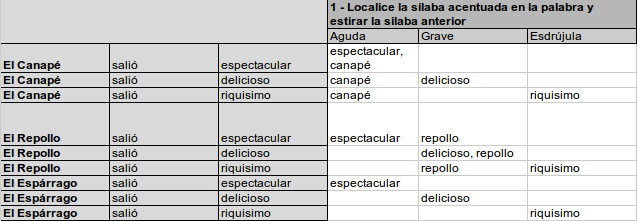
\includegraphics[width=1\textwidth]{reglas_AMPER} }
%    \caption{Frases AMPER}
%    \label{fig21}
%\end{figure}

\scriptsize
\begin{longtable}{| p{0.15\textwidth} | p{0.08\textwidth} | p{0.15\textwidth} || p{0.15\textwidth} | p{0.15\textwidth} | p{0.15\textwidth} |} 
	\hline
	%\multicolumn{6}{| p{0.9\textwidth} |} {\textbf{1 - Localice la sílaba acentuada en la palabra y estirar la sílaba anterior}} \\ \hline
	\multicolumn{3}{| p{0.45\textwidth} ||}{Frase} & \textbf{Aguda} & \textbf{Grave} & \textbf{Esdrújula} \\ \hline 
	\textit{El canapé} & \textit{salió} & \textit{espectacular} & espectacular, canapé & & \\ \hline
	\textit{El canapé} & \textit{salió} & \textit{delicioso} & canapé & delicioso & \\ \hline
	\textit{El canapé} & \textit{salió} & \textit{riquísimo} & canapé & & riquísimo \\ \hline
	\textit{El repollo} & \textit{salió} & \textit{espectacular} & espectacular & repollo & \\ \hline
	\textit{El repollo} & \textit{salió} & \textit{delicioso} &  & repollo, delicioso & \\ \hline	
	\textit{El repollo} & \textit{salió} & \textit{riquísimo} & & repollo & riquísimo \\ \hline
	\textit{El espárrago} & \textit{salió} & \textit{espectacular} & espectacular & & \\ \hline
	\textit{El espárrago} & \textit{salió} & \textit{delicioso} & & delicioso & \\ \hline
	\textit{El espárrago} & \textit{salió} & \textit{riquísimo} & & & riquísimo \\ \hline	
		
	\caption{Frases AMPER} 
	\label{fig21table}
\end{longtable}

\normalsize
\subsection{Frases comunes}

Como afirmamos antes, se utilizaron frases comunes para poder obtener los acentos de cada grupo de forma natural. Se pensó que si se graba una frase popular, el hablante al estar acostumbrado a decirla no iba a poder evitar impregnarle su acento. Todas las frases utilizadas se pueden ver en la tabla \ref{fig22tabla}.

%\begin{figure}[h!]
%    \centerline{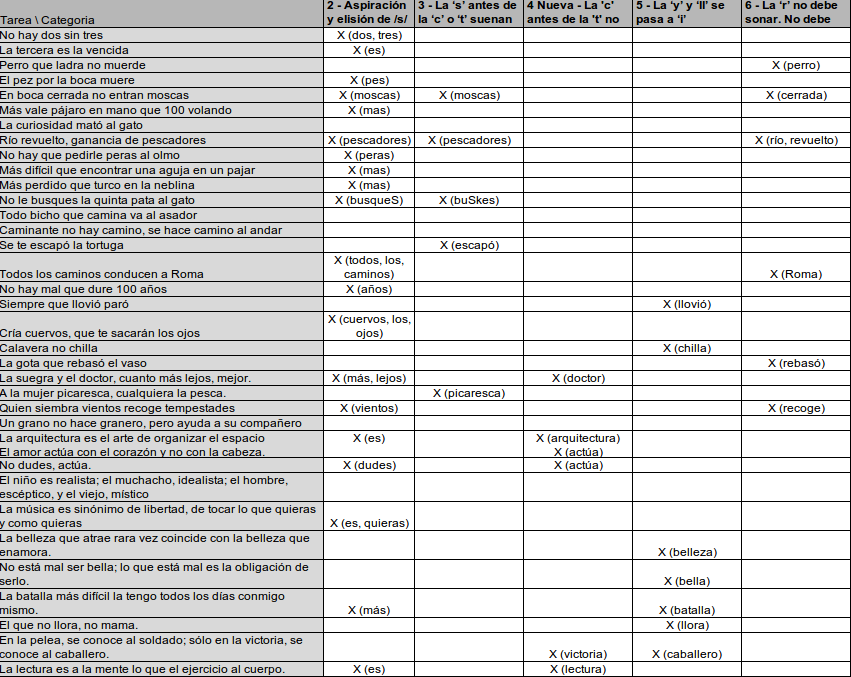
\includegraphics[width=1\textwidth]{frases_inf} }
%    \caption{Frases conocidas}
%    \label{fig22}
%\end{figure}

\newgeometry{margin=2cm} 
\begin{landscape}
\scriptsize
\begin{longtable}{| p{0.5\textwidth} || p{0.15\textwidth} | p{0.15\textwidth} | p{0.15\textwidth} | p{0.15\textwidth}| p{0.15\textwidth} | } 
	\hline
	\textbf{Frase} & \textbf{2 - Aspiración y elisión de /s/} & \textbf{3 - La 's' antes de la 'c' o 't' no suenan} & \textbf{4 - La 'c' antes de la 't' no suenan}& \textbf{5 - La 'y' y 'll' se pasa a 'i'} & \textbf{6 - La 'r' no debe sonar} \\ \hline	
	
	
	'No hay dos sin tres' & dos, tres & & & & \\ \hline
	'Más difícil que encontrar una aguja en un pajar' & más &&&& \\ \hline
	'Más perdido que turco en la neblina' & más &&&&  \\ \hline
	'No le busques la quinta pata al gato' & busques & busques &&&  \\ \hline
%	'Todo bicho que camina va al asador' &  \\ \hline
%	'Caminante no hay camino se hace camino al andar' &  \\ \hline
	'Se te escapó la tortuga' && escapó &&&  \\ \hline
	'Todos los caminos conducen a Roma' & todos, los, caminos &&&&  \\ \hline
	'No hay mal que dure cien anos' & años &&&& \\ \hline
	'Siempre que llovió paro' &&&& llovió & \\ \hline
	'Cría cuervos que te sacaran los ojos' & cuervos, los, ojos &&&&  \\ \hline
	'La tercera es la vencida' & es &&&& \\ \hline
	'Calavera no chilla' &&&& chilla &  \\ \hline
	'La gota que rebalsó el vaso' &&&&& rebasó \\ \hline
	'La suegra y el doctor cuanto más lejos mejor' & más, lejos & doctor&&& \\ \hline
	'A la mujer picaresca cualquiera la pesca' && picaresca &&&  \\ \hline
	'Quien siembra vientos recoge tempestades' & vientos &&&& recoge  \\ \hline
%	'Un grano no hace granero pero ayuda a su compañero' & \\ \hline
	'La arquitectura es el arte de organizar el espacio' & es && arquitectura && \\ \hline
	'El amor actúa con el corazón y no con la cabeza' &&& actúa&& \\ \hline
	'No dudes actúa' &&& actúa&&  \\ \hline
%	'El niño es realista; el muchacho, idealista; el hombre, escéptico, y el viejo místico' &  \\ \hline
	'Perro que ladra no muerde' &&&&& perro \\ \hline
	'La musica es sinónimo de libertad, de tocar lo que quieras y como quieras' & es, quieras &&&& \\ \hline
	'La belleza que atrae rara vez coincide con la belleza que enamora' &&&& belleza & \\ \hline
	'No esta mal ser bella lo que esta mal es la obligación de serlo' &&&& bella & \\ \hline
	'La batalla más difícil la tengo todos los días conmigo mismo' & más &&& batalla & \\ \hline
	'El que no llora no mama' &&&& llora & \\ \hline
	'En la pelea se conoce al soldado solo en la victoria se conoce al caballero' &&& victoria & caballero &\\ \hline
	'La lectura es a la mente lo que el ejercicio al cuerpo' & es && lectura &&  \\ \hline
	'El pez por la boca muere' & pez &&&& \\ \hline
	'En boca cerrada no entran moscas' & moscas & moscas &&& cerrada  \\ \hline
	'Más vale pájaro en mano que cien volando' & más &&&& \\ \hline
%	'La curiosidad mató al gato' &  \\ \hline
	'Río revuelto ganancia de pescadores' & pescadores & pescadores &&& río, revuelto  \\ \hline
	'No hay que pedirle peras al olmo' & peras &&&& \\ \hline
	
	\caption{Frases conocidas} 
	\label{fig22tabla}
\end{longtable}
\end{landscape}
\restoregeometry

\normalsize

Algo interesante es que una misma frase puede extraer atributos para varias reglas. Por ejemplo: la frase \textit{`En la pelea se conoce al soldado, sólo en la victoria se conoce al caballero’} extrae atributos para las reglas 4 y 5. La palabra \textit{`victoria’} cubre la regla 4 que nos propone medir la duración de la \textit{/c/} antes de la \textit{/t/}. Sucede igual con la palabra \textit{`caballero’} para la regla 5: el fonema \textit{/ll/} se pasa a \textit{/i/} cambiando su duración y sonido. En la Tabla \ref{fig22tabla} podemos ver que la cantidad de frases utilizadas con respecto a sus reglas es despareja. Hay más frases para la regla 2 que para las demás. Más adelante veremos como impacta esto en las frases que vamos a pedir grabar.

\subsubsection{Orden de las frases}

Ya definimos cuáles van a ser las frases, ahora debemos definir qué frases y en qué orden se deben decir durante el experimento. Diremos que una frase cubre una determinada regla si esta la satisface. Sucede que el orden que utilicemos va a ser crucial para obtener muestras: no es lo mismo empezar por una frase que sólo cubre una sola regla que varias. Si elegimos primero las frases que cubren varias reglas a la vez, en un sólo audio podremos obtener más cubrimiento de reglas. 

¿Por qué quisiéramos cubrir más reglas en una misma frase? Más adelante veremos que una frase grabada que cubre una regla aportará información sobre el hablante de esa regla en particular. Si una frase cubre varias reglas estaríamos obteniendo más información sólo utilizando una grabación. Por eso es importante maximizar el cubrimiento de las frases.  

El orden de las frases sigue el siguiente algoritmo:

\lstset{ %
language=C++,                % choose the language of the code
basicstyle=\footnotesize,       % the size of the fonts that are used for the code
numbers=left,                   % where to put the line-numbers
numberstyle=\footnotesize,      % the size of the fonts that are used for the line-numbers
stepnumber=1,                   % the step between two line-numbers. If it is 1 each line will be numbered
numbersep=5pt,                  % how far the line-numbers are from the code
backgroundcolor=\color{white},  % choose the background color. You must add \usepackage{color}
showspaces=false,               % show spaces adding particular underscores
showstringspaces=false,         % underline spaces within strings
showtabs=false,                 % show tabs within strings adding particular underscores
frame=single,           % adds a frame around the code
tabsize=2,          % sets default tabsize to 2 spaces
captionpos=b,           % sets the caption-position to bottom
breaklines=true,        % sets automatic line breaking
breakatwhitespace=false,    % sets if automatic breaks should only happen at whitespace
escapeinside={\%*}{*)},          % if you want to add a comment within your code
morekeywords={GeneradorDeTest, GenradorDeTrazas, checkBalance, Input, Output, Repetir, veces, Si, agregar, Recorrer, Devolver, y, no, esta, en, Mientras},
}
\begin{lstlisting}
    OrdenDeFrasesConocidas:
    Input: Frases (conj. String)
    Output: listaFrases (lista de String)
    listaFrases = {}
    DicPct <- Diccionario de porcentajes de cada regla
    Mientras Frases != {}:
    	regla <- ObtenerReglaConMenorPorcentaje(DicPct)
    	frase <- Frases.SacarLaMasPonderada(regla)
    	listaFrases.agregar(frase)
    	RecalcularPorcentajes(DicPct)
    Devolver listaFrases
\end{lstlisting}

%Texto viejo primera entrega
%La idea del algoritmo es la siguiente: vamos a utilizar un contador que nos va a decir cuántas muestras tenemos por cada regla. En cada paso vamos a ver ese contador y vamos a elegir la próxima frase teniéndolo en cuenta. Esta elección la lleva a cabo la función \textit{ObtenerLaMasPonderada}. Esta se encarga de elegir la frase que haga referencia a la regla menos grabada y además que represente a más de una regla. De esa forma intentamos obtener la mayor cantidad de información posible con pocas grabaciones y ponderamos las frases que referencien a más reglas. 

La idea del algoritmo es la siguiente: vamos a contabilizar la cantidad de muestras por cada regla. Esto se realiza calculando, para cada regla, la cantidad de frases que ya utilizamos cubriendo esa regla; sobre la cantidad total de frases que cubren esa regla. Entonces tendremos para cada regla su porcentaje de cubrimiento. Esto lo guardaremos en \textit{DicPct}.

Mientras haya frases sin ser seleccionadas para grabar, elegimos la regla que menos está cubierta. O sea, elegiremos como próxima regla a cubrir la que tenga menor porcentaje de cubrimiento. Esto se realiza en la función \textit{ObtenerReglaConMenorPorcentaje} utilizando como parámetro \textit{DicPct}.

Tenemos definida la próxima regla a cubrir. Debemos elegir la frase que cubra esa regla. Recordemos que hay muchas frases que cubren una determinada regla. Para definir cuál frase elegir vamos a optar por la que cubra mayor cantidad de reglas. Si hay varias frases en esta situación, elegimos una de estas al azar. Entonces no sólo aumentamos la cantidad de frases de la regla menos cubierta, sino que con esa frase cubrimos otras reglas. Esto se realiza en la función \textit{ObtenerLaMásPonderada}.

Para terminar, agregamos la frase elegida y recalculamos los porcentajes de cada regla en las lineas 9 y 10.

Esta idea es importante ya que llevamos al máximo la cantidad de información en cada frase y al hablante le hacemos perder menos tiempo realizando el experimento. Esto se puede ver en la Figura \ref{figFracesTraza} que representa el porcentaje de frases completadas mientras se va aumentando la cantidad de grabaciones. Teniendo en cuenta este algoritmo podemos notar que aproximadamente a partir de 10 grabaciones ya tenemos un buen porcentaje de cubrimiento. Por ejemplo, en la décima grabación la regla 4 ya tiene el 75\% de sus frases ya grabadas. La regla 5 el 50\% de sus frases ya grabadas. O sea, en la grabación número 10 ya se grabó alrededor del 40\% de la cantidad total de frases para cada regla.

TODO: escribir ejemplo
{\tiny \begin{table}[H]
	\centering
	\begin{tabular}{|l|l|c|c|c|c|c|}
		\hline
		 \textbf{Tarea}  & \textbf{Nro de Frase} &  \textbf{Regla 2} & \textbf{Regla 3} & \textbf{Regla 4} & \textbf{Regla 5} & \textbf{Regla 6} \\ \hline
		1 & 0 & 0\% & 0\% & 0\% & 0\% & 0\%\\ \hline
		2 & 24 & 5\% & 0\% & 0\% & 0\% & 20\% \\ \hline
		3 & 5 & 11\% & 25\% & 0\% & 0\% & 20\% \\ \hline
		4 & 26 & 17\% & 25\% & 25\% & 0\% & 20\%\\ \hline
		5 & 20 & 17\% & 25\% & 25\% & 50\% & 20\%\\ \hline
		6 & 22 & 23\% & 25\% & 50\% & 50\% & 20\%\\ \hline
		7 & 16 & 29\% & 25\% & 50\% & 50\% & 40\%\\ \hline
		8 & 8 & 35\% & 50\% & 50\% & 50\% & 40\%\\ \hline
		9 & 28 & 41\% & 50\% & 75\% & 50\% & 40\%\\ \hline
		10 & 21 & 41\% & 50\% & 75\% & 50\% & 60\%\\ \hline
		11 & 1 &  47\% & 50\% & 75\% & 50\% & 60\%\\ \hline
		12 & 2 &  52\% & 50\% & 75\% & 50\% & 60\%\\ \hline
		13 & 23 & 52\% & 75\% & 75\% & 50\% & 60\%\\ \hline
		14 & 18 & 52\% & 75\% & 75\% & 100\% & 60\%\\ \hline
		15 & 4 &  58\% & 75\% & 75\% & 100\% & 60\%\\ \hline
		16 & 6 &  64\% & 75\% & 75\% & 100\% & 60\%\\ \hline
		17 & 3 &  64\% & 75\% & 75\% & 100\% & 80\% \\ \hline
		18 & 9 &  70\% & 75\% & 75\% & 100\% & 80\%\\ \hline
		19 & 11 & 76\% & 75\% & 75\% & 100\% & 80\%\\ \hline
		20 & 15 & 76\% & 100\% & 75\% & 100\% & 80\%\\ \hline
		21 & 27 & 76\% & 100\% & 100\% & 100\% & 80\%\\ \hline
		22 & 10 & 82\% & 100\% & 100\% & 100\% & 80\% \\ \hline
		23 & 7 &  82\% & 100\% & 100\% & 100\% & 100\% \\ \hline
		24 & 12 & 88\% & 100\% & 100\% & 100\% & 100\%\\ \hline
		25 & 19 & 94\% & 100\% & 100\% & 100\% & 100\% \\ \hline
		26 & 30 & 100\% & 100\% & 100\% & 100\% & 100\% \\ \hline
	\end{tabular}
	\caption{}
	\label{}
\end{table}
}
%\begin{figure}[h!]
%    \centerline{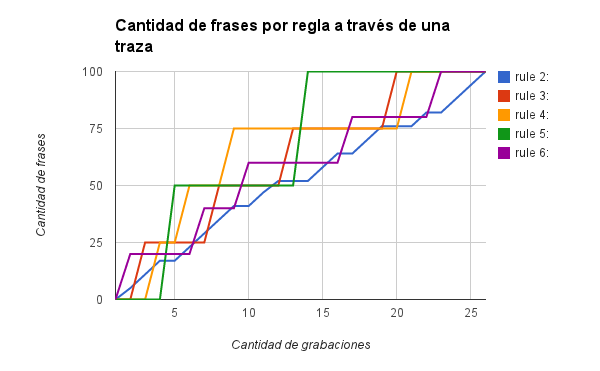
\includegraphics[width=0.9\textwidth]{cant_frases_traza_inf} }
    %\caption{Cantidad de frases por traza}
    %\label{figFracesTraza}
%\end{figure}

\begin{figure}[H]
	\centering
	\begin{tikzpicture}
	\begin{axis}[
	width=14cm,
	height=10cm,
	title={Porcentaje del total de frases por regla},
	xlabel={Cantidad de grabaciones},
	ylabel={Porcentaje del total de frases},
	xmin=0, xmax=25,
	ymin=0, ymax=100,
	xtick={0,5,10,15,20,25,30},
	ytick={0, 25, 50, 75, 100},
	legend pos=south east,
	ymajorgrids=true,
	xmajorgrids=true,
	grid style=dashed
	] 
	
	\addplot [mark=times*, line width=0.5pt]
	coordinates {
  		(0,0)(1, 0)(2, 5)(3, 11)(4, 17)(5, 17)(6, 23)(7, 29)(8, 35)(9, 41)(10, 41)(11, 47)(12, 52)(13, 52)(14, 52)(15,58)(16, 64)(17, 64)(18, 70)(19, 76)(20, 76)(21, 76)(22, 82)(23, 82)(24, 88)(25, 94)(26, 100)
	};\addlegendentry{Regla 2};
	
	\addplot [mark=times*, dash pattern=on 10pt off 5pt, line width=0.5pt]
	coordinates {
		(0,0)(1,0)(2,0)(3,25)(4,25)(5,25)(6,25)(7,25)(8,50)(9,50)(10,50)(11,50)(12,50)(13,75)(14,75)(15,75)(16,75)(17,75)(18,75)(19,75)(20,100)(21,100)(22,100)(23,100)(24,100)(25,100)(26,100)
	};\addlegendentry{Regla 3};
	
	\addplot [mark=times*, line width=2pt] 
	coordinates {
		(0,0)(1, 0)(2, 0)(3, 0)(4, 25)(5, 25)(6, 50)(7, 50)(8, 50)(9, 75)(10, 75)(11, 75)(12, 75)(13, 75)(14, 75)(15,75)(16, 75)(17, 75)(18, 75)(19, 75)(20, 75)(21, 100)(22, 100)(23, 100)(24,100)(25,100)(26, 100)
	};\addlegendentry{Regla 4};
	
	\addplot [mark=times*, dash pattern=on 10pt off 5pt, line width=2pt]
	coordinates {
		(0,0)(4,0)(5,50)(13,50)(14,100)(26,100) 
	};\addlegendentry{Regla 5};
	
	\addplot [mark=times*, dotted, line width=2pt] 
	coordinates {
		(0,0)(2,20)(6,20)(7,40)(9,40)(10,60)(16,60)(17,80)(22,80)(23,100) 
	};\addlegendentry{Regla 6};
		
		
%%		Tarea	rule 2:	rule 3:	rule 4:	rule 5:	rule 6:
%		1	0	0	0	0	0
%		2	5	0	0	0	20
%		3	11	25	0	0	20
%		4	17	25	25	0	20
%		5	17	25	25	50	20
%		6	23	25	50	50	20
%		7	29	25	50	50	40
%		8	35	50	50	50	40
%		9	41	50	75	50	40
%		10	41	50	75	50	60
%		11	47	50	75	50	60
%		12	52	50	75	50	60
%		13	52	75	75	50	60
%		14	52	75	75	100	60
%		15	58	75	75	100	60
%		16	64	75	75	100	60
%		17	64	75	75	100	80
%		18	70	75	75	100	80
%		19	76	75	75	100	80
%		20	76	100	75	100	80
%		21	76	100	100	100	80
%		22	82	100	100	100	80
%		23	82	100	100	100	100
%		24	88	100	100	100	100
%		25	94	100	100	100	100
%		26	100	100	100	100	100
		
	\end{axis}
	\end{tikzpicture}
    \caption{Porcentaje del total de frases grabadas por cada regla}
    \label{figFracesTraza}
\end{figure}


\subsection{Combinando los dos tipos de frases utilizando trazas}

Definimos frases comunes y AMPER para grabar. Ahora debemos definir cómo vamos a ir intercalando cada tipo en el experimento. Para ello definimos traza. Una traza es una lista de las frases que va a grabar un hablante en el experimento. Esta va a estar compuesta entre 1 a 3 frases comunes extraídas del orden definido en \textit{OrdenDeFrasesConocidas}, y luego una frase del esquema de AMPER. Tanto la cantidad de frases comunes como la elección de la frase AMPER se realiza al azar. Este patrón se repite sucesivamente hasta completar todas las frases. La idea es no cansar al hablante con frases repetitivas y evitar que sepa de antemano qué frase va a tener que grabar ya que si fuera el caso, podría exagerar la entonación.

Al empezar el experimento, al hablante se le dará una traza que grabará sucesivamente en ese orden. Elegimos tener precalculadas las trazas para evitar cálculos costosos a la hora de empezar el experimento. Si no se precalcularan las trazas, deberíamos realizar los cálculos cada vez que empieza el experimento y podríamos retrasar la grabación del hablante. Es por eso que guardamos 10.000 trazas generadas. 

La mínima cantidad de grabaciones que puede realizar un hablante son 5 grabaciones. Luego se le pregunta si quiere continuar grabando. Si acepta, se le agregan otras 5 grabaciones así sucesivamente hasta llegar al total de frases a grabar. Elegimos grabar cada 5 grabaciones para que el hablante aporte el tiempo que tenga disponible y no obligarlo a grabar todas las frases. Aunque no grabe la totalidad de frases, las muestras van a servir en el experimento.

A continuación veremos cómo implementamos el sistema de grabación para soportar este experimento.
\chapter{Sistema de grabación online}

Para poder obtener audios de distintas personas se desarrolló una página web. Esto nos da mucha ventaja ya que nos permite grabar fácilmente desde cualquier lugar. En esta sección explicaremos la arquitectura del sistema y sus detalles técnicos.

La página web está desarrollada en Django, versión 1.4.2. Se eligió este framework por su facilidad a la hora de guardar objetos a la base de datos y también por la cantidad importante de bibliotecas que posee Python. La versión de Python que se utilizó es 2.7.3. 

En la base de datos se guarda la información de cada hablante, las frases a grabar y las trazas. La base de datos elegida fue PostgreSQL versión 9.1 y se escogió esta ya que es de código abierto. Los archivos de audio se guardan en archivos \textit{wav} por separado y también se guarda una referencia al nombre del archivo generado en la base de datos. Para el servidor HTTP se utiliza Apache versión 2.2.22. El servidor utiliza el sistema operativo Ubuntu 12.04.4 LTS.

\section{Recolección de datos}

Cuando un usuario visita nuestra página, primero debe llenar un formulario. Este le pregunta: género, fecha de nacimiento, lugar donde se crió y donde reside actualmente. Al confirmar el formulario, estos son grabados en la base de datos de la aplicación en el servidor. Esto se puede apreciar en la Figura \ref{figEncuesta}. Luego se procede a realizar las grabaciones. 

\begin{figure}[h!]
    \centerline{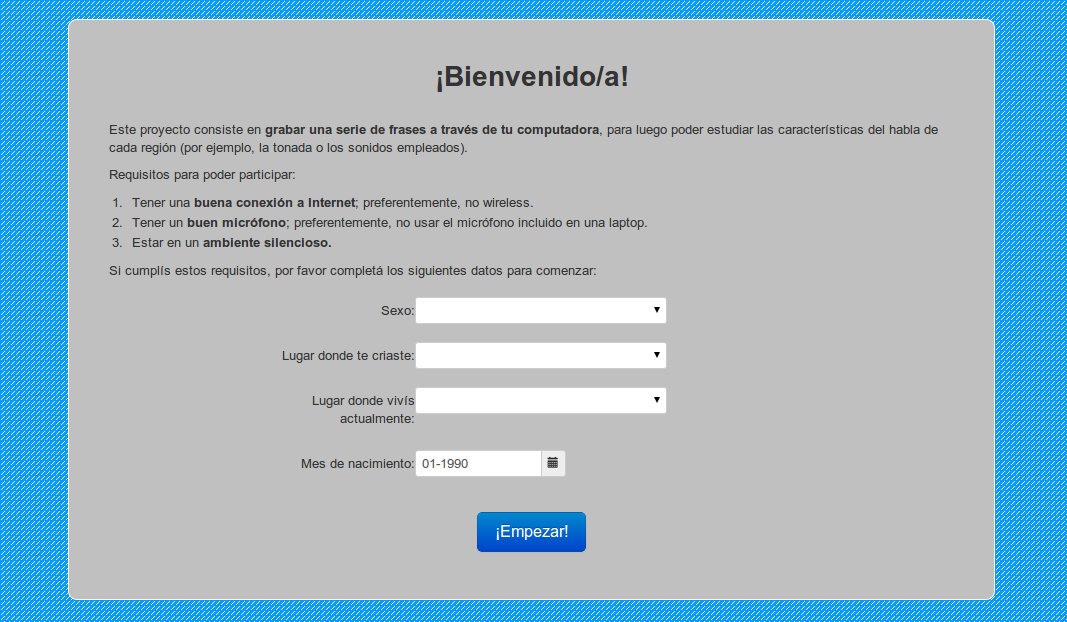
\includegraphics[width=0.8\textwidth]{pag-inicio2} }
    \caption{Encuesta inicial del sistema}
    \label{figEncuesta}
\end{figure}

\begin{figure}[h!]
    \centerline{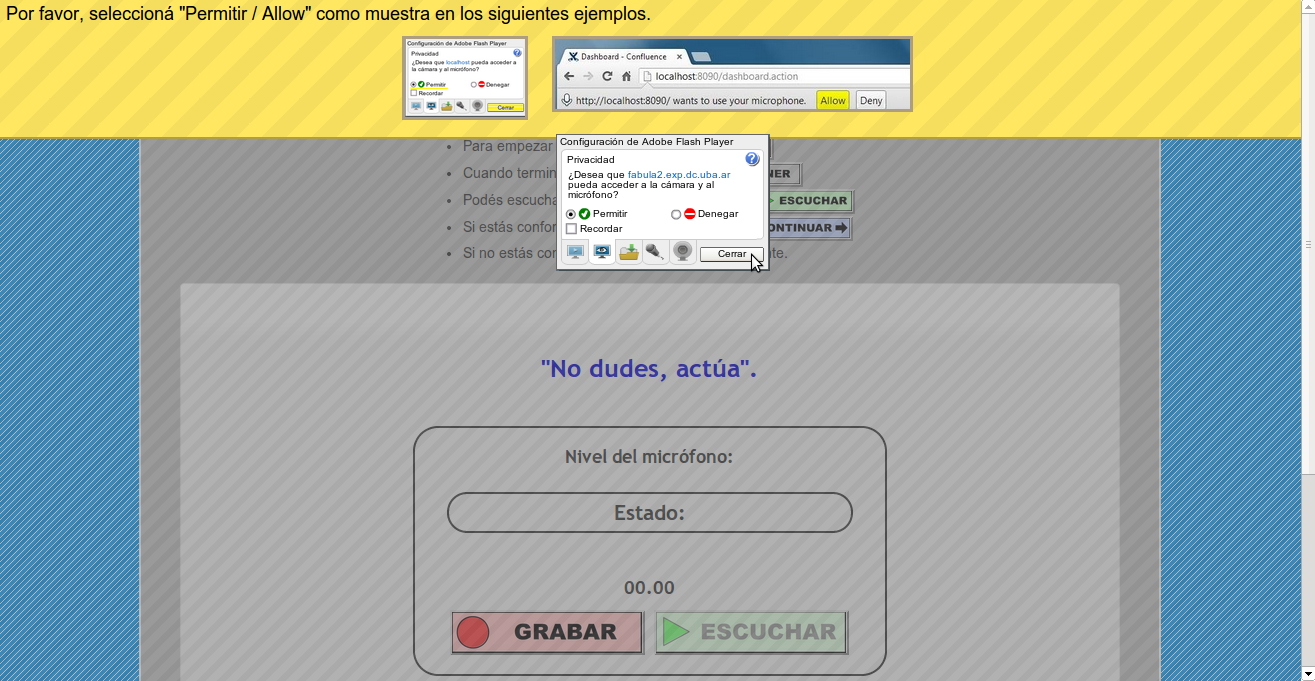
\includegraphics[width=0.8\textwidth]{pag-allow1} }
    \caption{Se debe permitir micrófono para comenzar el experimento}
    \label{allowmic}
\end{figure}

\begin{figure}[h!]
    \centerline{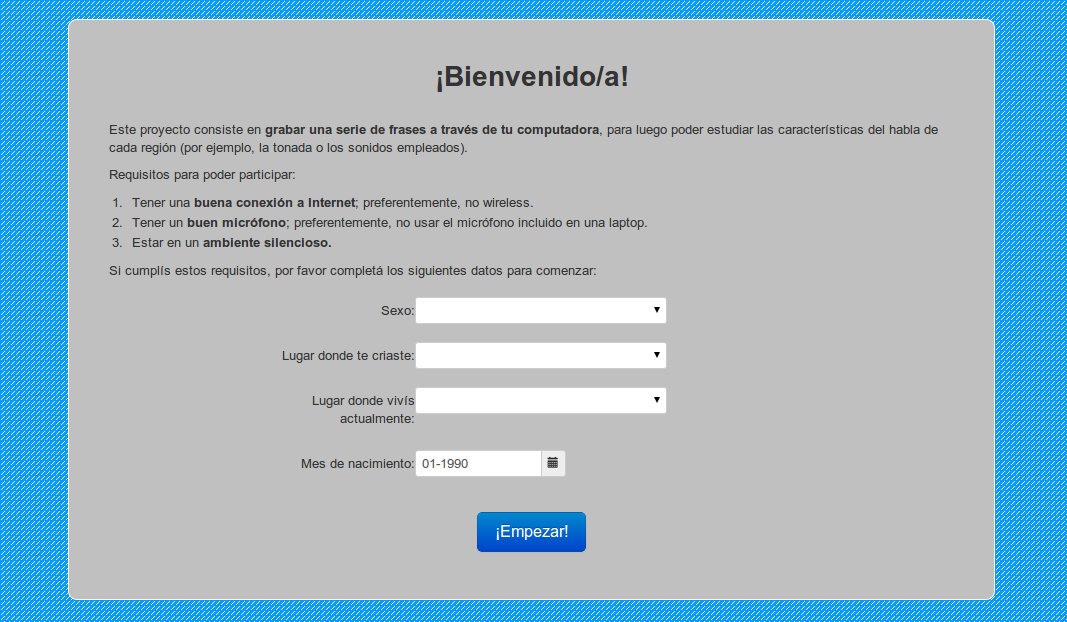
\includegraphics[width=0.8\textwidth]{pag-inicio2} }
    \caption{Inicio del experimento}
    \label{inicio}
\end{figure}

\begin{figure}[h!]
    \centerline{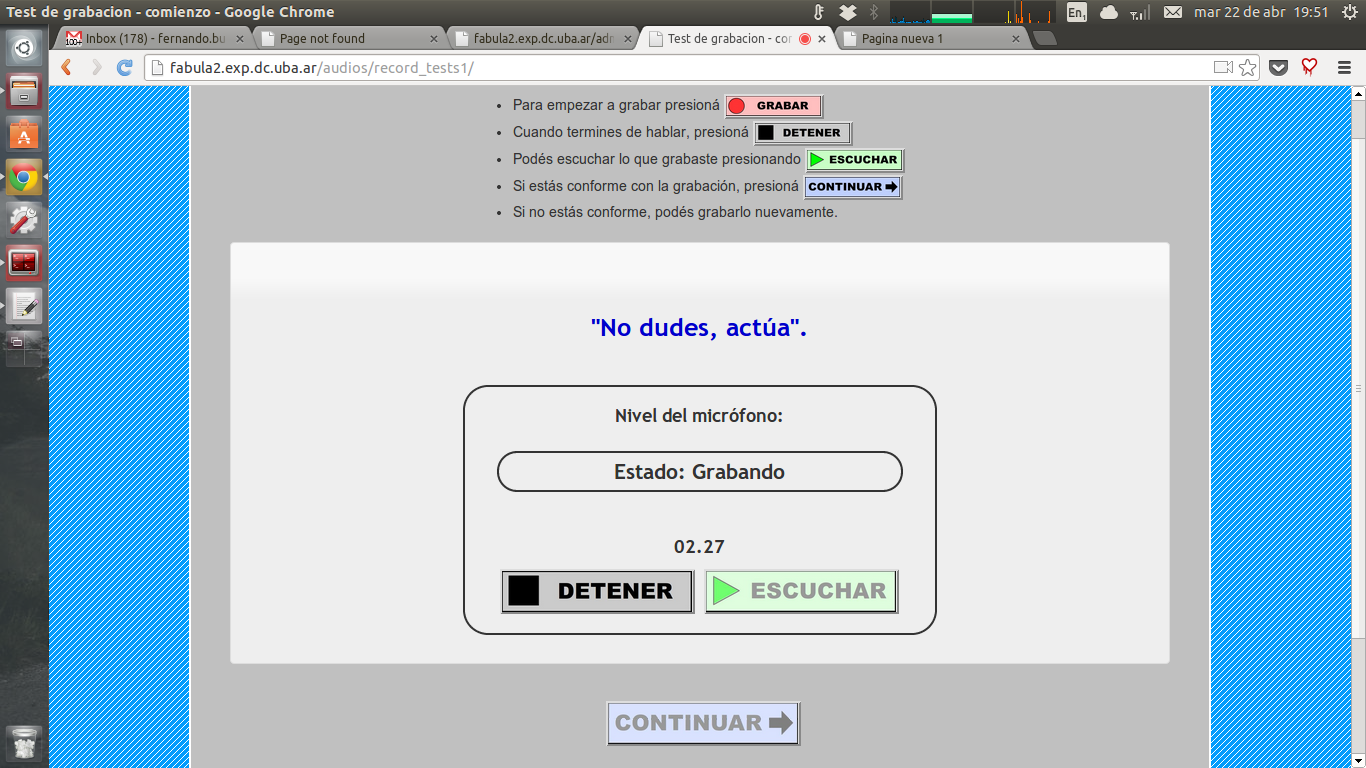
\includegraphics[width=0.8\textwidth]{pag-grabar1} }
    \caption{Grabando una frase}
    \label{grabando}
\end{figure}

\begin{figure}[h!]
    \centerline{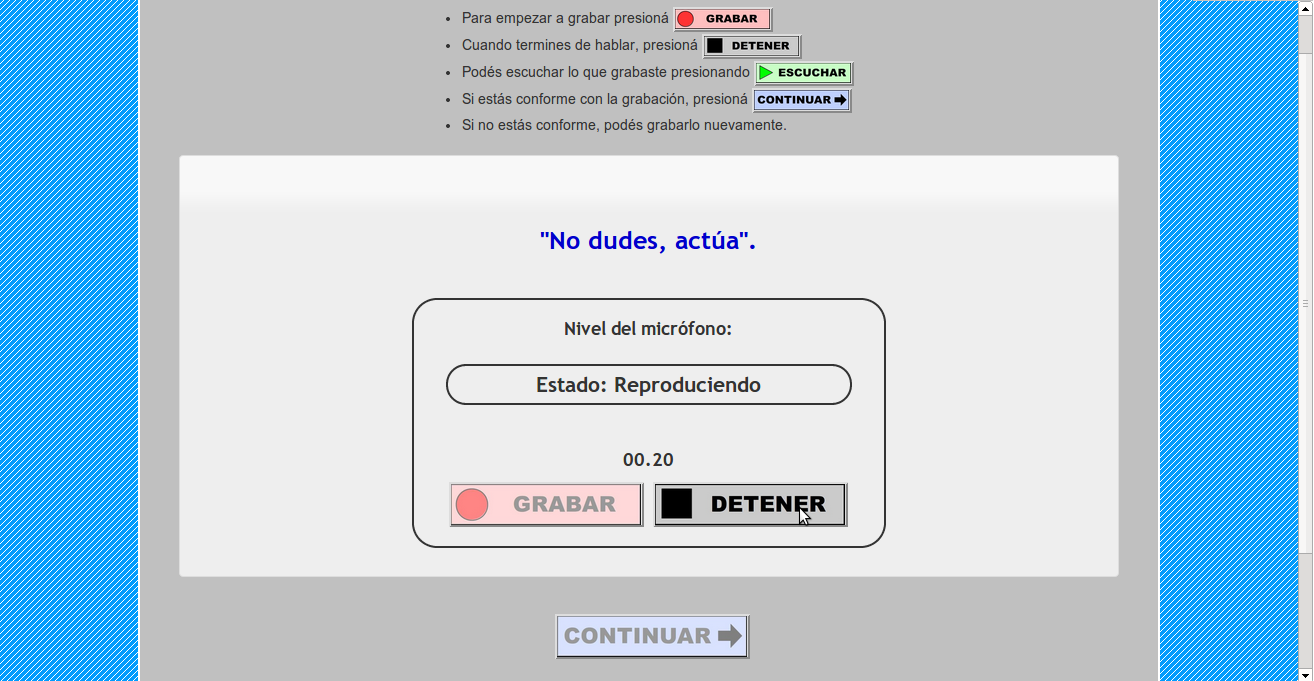
\includegraphics[width=0.8\textwidth]{pag-play1} }
    \caption{Reproduciendo la frase anteriormente grabada}
    \label{reproduciendo}
\end{figure}

En la pantalla de grabación el usuario debe confirmar el acceso al micrófono que posee en su computadora, como se puede apreciar en la Figura \ref{allowmic}. Una vez hecho esto, se le explica las instrucciones del experimento, como se ve en la Figura \ref{inicio} y luego puede empezar a grabar. 

Cada nuevo experimento utiliza una nueva traza del conjunto de trazas descriptas en la capitulo anterior. La interfaz que ve el usuario al grabar cada frase se puede ver en la Figura \ref{grabando}. Las grabaciones pueden ser escuchadas por el usuario. Si el usuario al escucharla nota que no es una buena grabación, tiene la posibilidad de grabarla otra vez. Lo importante es que la última grabación se escuche lo mejor posible. Para que el usuario reproduzca su grabación se aprieta en el botón \textit{Reproducir} como se ve en la figura \ref{reproduciendo}. 

Una vez que el hablante cree que su grabación se escucha bien, la confirma. Cada vez que se graba un audio, este se guarda en un archivo wav en el servidor. El archivo que se genera tiene una frecuencia de muestreo de 22050 Hz, cada muestra se analiza con 16 bits y posee un solo canal. Con estas características pudimos obtener un audio de buena calidad para el experimento que realizamos.

Recordemos que los hablantes graban en series de 5 frases. Una vez terminado estas 5 frases se le pregunta si quiere seguir grabando o terminar el experimento. De esta forma, el hablante aporta el tiempo que puede disponer.

\section{Grabación a través del browser}

Los navegadores actuales no permiten acceder al micrófono directamente. Actualmente se desarrolla HTML5 que permitirá acceder al micrófono y a recursos similares de forma más fácil. No se eligió basarse en este porque sólo los browsers más nuevos lo soportan. Al ser un estándar muy nuevo necesita que el usuario tenga instalada últimas versiones de software y utilizarlo hubiera excluido mucha gente. Teniendo en cuenta esto debimos utilizar una tecnología alternativa. 

Encontramos un proyecto llamado Web Accessible Multimodal Interfaces \footnote{Página web: https://code.google.com/p/wami/} (WAMI). WAMI es una aplicación Flash que nos permite acceder al micrófono a través de JavaScript. El proyecto WAMI es muy utilizado en proyectos similares de procesamiento de habla. Esta herramienta nos permite definir dos URLs importantes: una que se utilizará para enviar el audio grabado y otra para escucharlo.  

Cuando termina de grabar, se envía un mensaje POST al servidor a la URL configurada. El servidor obtiene el paquete de información y lo guarda como archivo wav. Cuando se quiere reproducir algún audio se envía un mensaje GET a la otra URL. El servidor lo responde con el audio requerido y se reproduce en el navegador. También con WAMI se puede configurar la calidad del audio grabado y analizar el nivel del volumen que posee. 

\subsection{Requerimientos}

Los requerimientos para participar del experimento son básicos: se debe disponer de micrófono y conexión a internet. Tuvimos problemas sobre el browser que se utilizaba: WAMI necesita Flash versión 11.04 que no se encuentra en los repositorios tradicionales de Ubuntu. De esta manera, los navegadores que utilicen Flash instalado por el sistema operativo Ubuntu no podrán correr. Otros sistemas operativos como Windows o MacOs no tienen problemas con la versión de Flash instalada. De todas formas el navegador Chrome posee preinstalado la última versión de Flash, con lo cual este navegador puede correr perfectamente la aplicación sin importar el sistema operativo que se utilice.

\section{Varias grabaciones por frase}

Recordemos que para tener la mejor grabación de cada frase, le dimos la opción al hablante de que pueda escuchar como quedó. Esto requiere un ida y vuelta de paquetes entre el cliente (navegador) y el servidor. 

Al grabar el cliente manda un mensaje al servidor con el audio de la grabación en crudo. Las frases son de corta longitud entonces no es necesario preocuparse por la longitud del paquete. Cuando el cliente quiere escucharlo envía un mensaje pidiendo ese mismo audio anteriormente grabado. El servidor envía el audio y es reproducido en el cliente. Este ida y vuelta de la grabación podría ser optimizada para que la grabación pueda ser escuchada sin tener interacción con el servidor. En nuestro experimento, no tuvimos problemas graves en lo que respecta a latencias pero es un punto débil del sistema que hay que tener en cuenta.

Puede resultar interesante analizar los anteriores audios grabados para ver por qué el hablante elige el último. Esta idea también puede motivar a algún trabajo futuro.

\section{Sistema de administración}

Además de la interfaz pública para grabar audios, implementamos un sistema privado para administrar las grabaciones. Este nos permite ver las grabaciones que fueron grabadas, la cantidad de grabaciones por cada frase que tenemos recolectada, la cantidad de trazas que todavía no se utilizaron, entre otras cosas. También nos permite escuchar y marcar las grabaciones para utilizarlas como primer filtro de las grabaciones. Explicaremos esto en más detalle a continuación.

\subsection{Etiquetado de audio}

Cuando varias personas terminan el experimento, los administradores pueden acceder a una página donde se puede escuchar cada audio que se va grabando. Los administradores escuchan las grabaciones y según su calidad los etiquetan con alguna de las etiquetas definidas. Las etiquetadas utilizadas esta vez son: `Conservar’,  `Sonido saturado’, `Mucho ruido de fondo’, `Problemas en el habla’. Esto se puede ver en Figura \ref{cat}.

\begin{figure}[h!]
    \centerline{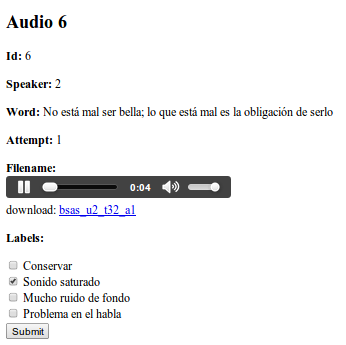
\includegraphics[width=0.5\textwidth]{categorizando_audios} }
    \caption{Categorizando audios}
    \label{cat}
\end{figure}

Para acceder a los audios que fueron etiquetados de una determinada manera, el sistema tiene distintas URLs que nos permiten bajar todos esos audios en un archivo de tipo tar. Entonces si quisiéramos bajar todo el audio etiquetado con la categoria `Conservar’ podemos acceder a una url y bajarnos sin necesidad de entrar al servidor. Se necesita ser usuario del sistema para poder acceder a este sistema.

\section{Backups automáticos}

El sistema posee backups que se generan a la noche automáticamente. Los backups consisten en un volcado de información de toda la base de datos y en la sincronización de las grabaciones con una carpeta externa de backup.

\section{Análisis del volumen}

Un requerimiento primordial de este experimento es evitar grabaciones saturadas. Para ello medimos el volumen de la grabación mientras esta se produce. El resultado es una serie de valores entre 0 a 100. Sobre estos valores calculamos el máximo y el mínimo. Si el primero es mayor a un cierto umbral arbitrario (o sea mayor a 80 por ejemplo) significa que la grabación saturó en algún momento. Si el mínimo es mayor a un cierto umbral (o sea menor a 20 por ejemplo) quiere decir que hay mucho ruido ambiente. En cualquiera de los dos casos podemos pedirle al usuario que grabe nuevamente el experimento. De esta forma podemos filtrar grabaciones que no nos servirán para reconocer el acento.

Si bien la característica de filtrar por volumen fue programada, no fue utilizada en este experimento. El motivo fue que queríamos chequear cuán bien funcionaba la herramienta sin filtros y con completa participación de los usuarios. Otro motivo fue la paciencia de los hablantes: puede suceder no logre un ambiente beneficioso para grabar y, aunque quiera, el filtro rechace todos sus audios. También notamos que había grabaciones que dieron mal el filtrado del volumen pero la grabación era buena. Esto no lo queremos como primer experimento del framework. Por eso elegimos aceptar todas las grabaciones.

A continuación veremos como utilizamos esta información recolectada para el objetivo del experimento.
\chapter{Extracción de información}

Utilizando nuestra página web podemos obtener distintas muestras de Córdoba y Buenos Aires. ¿Cómo podemos analizar estas grabaciones correctamente? Un archivo wav, similar al que se genera en cada una de las muestras, posee muchísima información. Es por esto que debemos seleccionar correctamente qué partes de la información nos sirven y qué partes podemos descartar.

\section{Alineación forzada}

Una grabación a partir de una frase posee muchísima información. Debemos seleccionar qué parte de esta grabación nos interesa y qué parte puede ser descartada. Para ello etiquetamos en qué partes del audio se pronunció cada fonema y también, uniendo cada uno de estos fonemas, etiquetamos cada palabra. Por ejemplo: si tenemos la grabación de la frase \textit{`El canapé salió espectacular’}, utilizamos un archivo aparte que nos dice \textit{`<<espectacular>> se escucha entre el segundo 0.90 y 1.18’}. Lo mismo sucede para cada palabra y fonema de la grabación. Para marcar estas anotaciones utilizamos el formato de archivos TextGrid del programa Praat  \cite{praat}.

Un dato muy importante es que este etiquetado no debe tener que ser realizado con intervención de un humano. Si fuera el caso, tendríamos que hacerlo uno por uno, y al tener muchos audios sería un trabajo muy arduo. De esto se encarga la alineación forzada. Las partes que debemos extraer de los audios son donde se encuentran la diferencias de cada regla descripta anteriormente. 

\subsection{Prosodylab Aligner}

%If you use this tool, we would appreciate it if you cite the following paper:
%Gorman, Kyle, Jonathan Howell & Michael Wagner (2011). Prosodylab-Aligner: A tool for forced alignment of laboratory speech. Proceedings of Acoustics Week in Canada, Quebec City.

Debemos tener una herramienta que nos permita obtener estos pequeños fragmentos de audio para analizar sus diferencias. Usamos una, llamada ProsodyLab Aligner \cite{prosodylab}. Su función es realizar alineaciones automáticas en cada uno de los audios de forma fácil. Analiza uno por uno cada audio y mediante un diccionario determina en qué momento se dijo cada fonema y palabra. 
%(TODO CORRECCIÓN DE AGUSTÍN: no se entiende si tengo que borrar todo el párrafo o no)

%Como dijimos, el formato de archivo utilizado para devolver estas marcas es TextGrid. El problema de la alineación automática es un caso particular de la alineación de audios.

Una particularidad que se destaca de esta herramienta es que no necesita datos de entrenamiento. Sólo con una hora de grabación es suficiente para correrlo y obtener resultados. Otra característica es que puede utilizarse para cualquier idioma. Esta herramienta está hecha en lenguaje Python (versión 2.5) y sirve como $wrapper$ para utilizar HTK fácilmente. HTK es una librería para crear y manipular Modelos Ocultos de Markov fácilmente, y SoX, que nos permite trabajar con audio a través de la consola. 

%explicación teórica con ejemplo
\subsubsection*{Modelos ocultos de Markov}
Los Modelos Ocultos de Markov \cite{rabiner} (en ingles HMM) son modelos estadísticos por los cuales tratan de predecir parámetros ocultos a través de observaciones. Se llaman ``ocultos'' ya que el estado a predecir no se puede observar directamente. Sólo se puede predecir en qué estado oculto está a través de observaciones. 

Un ejemplo de este modelo podría ser predecir la presión atmosférica observando sólo si el tiempo está lluvioso o seco. Los estados ocultos serían ``Baja'' o ``Alta'' presión atmosférica, que corresponde a lo que queremos saber. Las observaciones para predecir estos estados serían ``Lluvia'' o ``Seco''. En la Figura \ref{ex_hmm} se puede apreciar este ejemplo. Para saber en qué estado oculto se encuentra a través de las observaciones se utiliza el algoritmo Viterbi.

\begin{figure}[htbp]
	\begin{center}
		\begin{tikzpicture}[]
		% states
		\node[state] (s1) at (-0.5,2.5) {$Baja$}
		edge [loop above] node[auto,swap,left=2] {$0.3$} ();
		\node[state] (s2) at (2.5,2.5) {$Alta$}
		edge [<-,bend right=40] node[auto,swap] {$0.7$} (s1)
		edge [->,bend left=40] node[auto,swap] {$0.2$} (s1)
		edge [loop above] node[auto,swap,right=2] {$0.8$} ();
		% observations
		\node[observation] (y1) at (-1,0) {$Lluvia$}
		edge [lightedge] node[auto,swap] {$0.6$} (s1)
		edge [lightedge] node[auto,swap] {$0.4$} (s2);
		\node[observation] (y2) at (3,0) {$Seco$}
		edge [lightedge] node[auto,swap] {$0.4$} (s1)
		edge [lightedge] node[auto,swap] {$0.6$} (s2);
		\end{tikzpicture}
	\end{center}
	\caption{HMM}
	\label{ex_hmm}
\end{figure}

%ejemplo de audio sobre el trabajo
Llevado esta idea a nuestro trabajo, los Modelos Ocultos de Markov tratan de predecir qué fonemas aparecen en cada parte de los audios utilizando la lista de fonemas pronunciada en cada grabación. Mediante este modelo matemático, el programa analiza en cuáles grabaciones, de la misma frase, se produce un mismo patrón de sonido. Si sucede esto en todas estas grabaciones, se lo marca como un fonema de la frase. Ese fonema va a ser marcado de igual forma en el TextGrid de cada una de las grabaciones. Los estados ocultos a predecir son los fonemas de cada frase, en cambio las observaciones provienen del análisis de cada audio. Entonces, a través de muestras va prediciendo los fonemas de las grabaciones.

Veamos un ejemplo de cómo funcionan los HMM en nuestro trabajo. 

\begin{figure}[H]
	\centering
	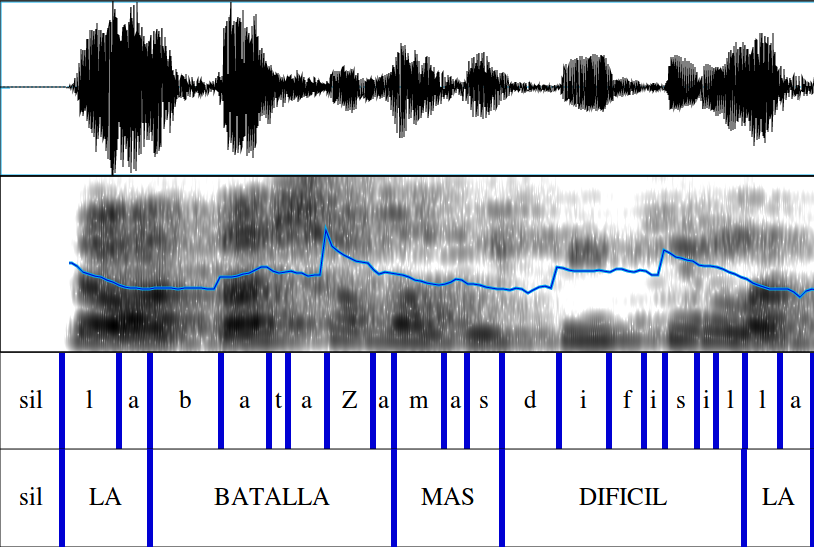
\includegraphics[width=0.8\textwidth]{espectograma_u3_t33_a1} 
	\caption{Características audio 1}
	\label{car_a1}
\end{figure}

\begin{figure}[H]
	\centering
	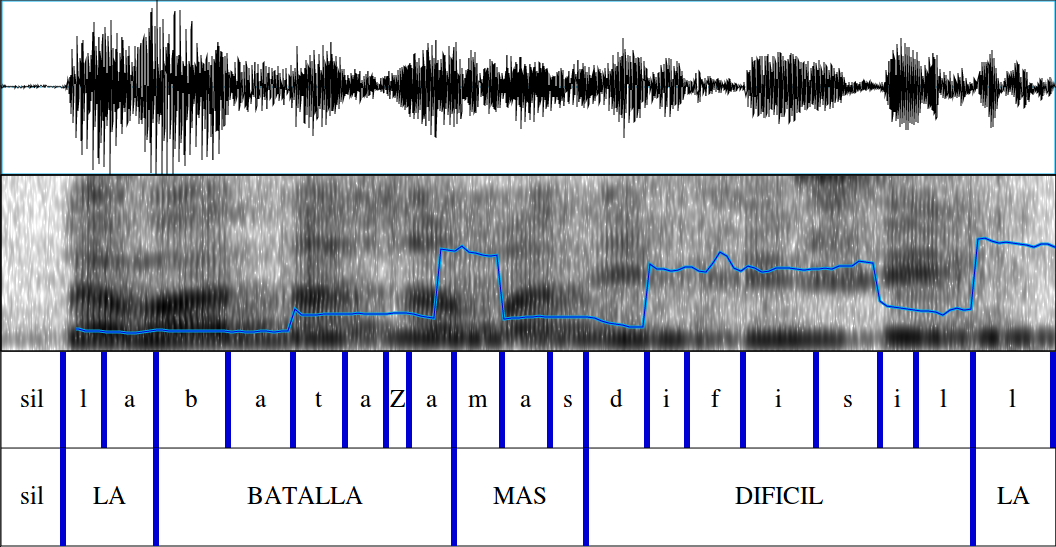
\includegraphics[width=0.8\textwidth]{espectograma_u27_t33_a1} 
	\caption{Características audio 2}
	\label{car_a2}
\end{figure}

Las imágenes \ref{car_a1} y \ref{car_a2} muestran las características de dos grabaciones, de dos hablantes distintos, que pronuncian la misma frase. Estas características están representadas por tres gráficos. El primero nos muestra la onda del sonido de la grabación a través del tiempo, el segundo el espectograma y el tercero corresponde al comienzo y fin de cada fonema en la grabación. 

Podemos observar que el espectograma de ambas grabaciones es muy distinto. Si comparamos la zona del espectograma que se encuentra el enésimo fonema con respecto al mismo fonema del otro espectograma, vemos que ambas son muy diferentes. Aún así la alineación de los fonemas es similar. Si bien no son zonas iguales, poseen similares valores de MFCC\footnote{Mel Frequency Cepstral Coefficients se verán cómo se calcular más adelante} para esa región. Los Modelos Ocultos de Markov analizan los coeficientes MFCC y teniendo en cuenta la sucesión de fonemas de la frase, que es similar para ambas grabaciones, puede predecir los tiempos de inicio y fin de cada fonema. De esta forma, puede predecir desde y hasta qué tiempo se encuentra cada fonema.
\\

Volviendo a nuestro sistema, los requisitos para utilizar ProsodyLab Aligner son: una hora de grabación con alineamientos y un diccionario fonético que nos provea para cada palabra los distintos fonemas que la componen. La hora de grabación la debíamos cumplir recolectando grabaciones de la página web. Esta meta era posible de realizar. La creación de un diccionario fonético era más complicado, ya que debía ser en español. Gracias al \textit{Laboratorio de Investigaciones Sensoriales} \footnote{Página web: http://www.lis.secyt.gov.ar/} que nos prestó un diccionario, implementado por ellos, pudimos utilizar esta herramienta. Un diccionario fonético es básicamente un listado con las palabras que utilizamos y su transcripción en fonemas. Es importante esto ya que va a ser usado por el alineador para describir los fonemas de cada palabra en cada frase.

%TODO: arreglar sin poner SCORES
%Una vez terminada la alineación, ProsodyLab Aligner genera un archivo donde muestra cómo fueron esas alineaciones utilizando un puntaje. Este archivo se llama \textit{`.SCORES’} y en él se encuentra una lista de todos los audios seguidos de un valor, corresponde a la verosimilitud de las alineaciones. Si una alineación fue similar a otra va a tener aproximadamente un valor similar. En cambio, si posee una alineación muy distinta va a tener valores muy distintos. Este puede ser el primer filtro para el extractor. 
%(TODO CORRECIÓN: PERO QUE ES ESA VEROSIMILITUD)

%Ordenando los audios utilizando esta numeración notamos que los menores poseen alineaciones malas, entonces definimos un umbral arbitrario para el cual aceptar la alineación si este se supera. Si bien este procedimiento es efectivo, notamos que se encuentran algunos falsos positivos, o sea archivos que tienen un buen punto de score pero la alineación es mala. Al tener pocas grabaciones no pudimos aceptar estos casos, debimos corregirlos uno por uno.

\section{Extracción de atributos}

La extracción de atributos fue realizada utilizando el lenguaje Python, que elegimos ya que es fácil de programar y tiene muchas librerías útiles para este tipo de casos. Utilizamos una librería muy conocida llamada Numpy (versión 1.6.1). Esta se utiliza para realizar cálculos matemáticos. Nosotros la utilizamos para tener buena precisión en el cálculo de los atributos.

Después de la alineación realizada, se ejecuta el extractor de atributos. Este posee como input los archivos Wav y TextGrid que corresponden a las alineaciones temporales de cada fonema en cada audio. El workflow del extractor se puede ver en la Figura \ref{workflow}. 

La rutina principal del programa toma una por una las grabaciones y su etiquetado asociado. Esta se representa en el componente ``Extractor''. Este llama a distintos componentes que van a calcular cada atributo. Para calcular estos atributos vamos a dividir en dos componentes: ``Acoustic Extractor'' que se encarga de extraer \textit{atributos acústicos} y ``TextGrid Extractor'' que se encarga de extraer \textit{atributos temporales}. Los atributos temporales son calculados solamente utilizando el TextGrid mientras que los atributos acústicos son calculados no sólo el TextGrid sino también el cálculo de MFCC, que veremos más adelante. Si el atributo está presente en la grabación tendremos ese dato en la extracción, si no se dejará como desconocido. Luego de calculado todos sus atributos paa cada grabación, juntamos todos los resultados y generamos el archivo Arff utilizando el componente ``Arff File Maker''.

El archivo Arff tiene por cada línea una grabación y seguido todos los resultados del cálculo de los atributos separado por comas. Necesitamos utilizar este formato ya que es necesario para ingresar datos en Weka, la plataforma que elegimos para correr algoritmos de \textit{machine learning}. Veamos cada uno de los dos tipos de atributos:

\begin{figure}[h!]
    \centerline{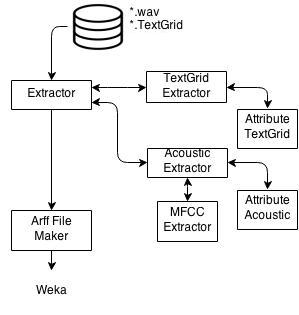
\includegraphics[width=0.5\textwidth]{diagrama_workflow} }
    \caption{Diagrama workflow}
    \label{workflow}
\end{figure}

\subsection{Atributos temporales}

Los atributos temporales corresponden a atributos sobre la duración de los fonemas y las sílabas de cada frase. Para calcularlos utilizamos como input el TextGrid generado en la alineación. Básicamente estas funciones recorren el TextGrid buscando un patrón en particular y miden su duración. Los atributos temporales se dividen en dos grupos: fonéticos y silábicos. 

Luego, las mediciones son normalizadas. Se realizan dos normalizaciones. La primera, conocida como z-score, será utilizando la forma:

\hspace{2cm} \[\frac{ X - \mu }{ \sigma }\]

\noindent donde:

\begin{itemize}
	\item $X$ es el valor a normalizar (por ejemplo: la duración de un fonema dado).
	\item $\mu$ es el promedio de duración de la unidad utilizada en la grabación.
	\item $\sigma$ es el desvío estándar de la unidad utilizada en la grabación.
\end{itemize}

\noindent Y luego la segunda suponiendo que $\mu = 0$:

\hspace{2cm} \[\frac{ X }{ \sigma }\]

\noindent Esta última tiene el nombre de Half-normal Distribution.

El valor a normalizar puede variar: mientras uno va a tener en cuenta fonemas, el otro tiene en cuenta sílabas. Debemos utilizar los datos normalizados ya que necesitamos atributos que nos muestren, para un hablante en particular, si el fonema en cuestión es relevante con respecto a los demás de la grabación. Al normalizar un atributo vemos cuán fuera de lo común resulta en el marco de \textit{ese} hablante en particular en \textit{esa} grabación. No importa si habla lento o rápido. Lo importante es la relación del fonema a medir con respecto a los demás. Lo mismo sucede para las sílabas. Si utilizáramos valores absolutos, se perdería esta relación ya que variaría con respecto a la velocidad del habla de cada hablante y cada grabación.
 
A continuación veamos los atributos en particular para cada uno de los grupos y cómo se realiza su cálculo. Para la regla 1 vamos a definir atributos silábicos, ya que corresponde a reglas que están definidas para sílabas, mientras que para las demás reglas (2 al 6) vamos a definir atributos fonéticos.

\subsubsection{Atributos fonéticos}

Los atributos que contabilizan fonemas son:

\begin{itemize}
    \item \textbf{Duración de `kt’:} en este atributo buscamos el patrón /kt/ en los TextGrids y luego, en ese intervalo, medimos la duración del fonema /k/. Este atributo intenta extraer la diferencia explicada en la regla 4, que nos indica la duración de dicho fonema.
    \item \textbf{Duración de `sc’:} ídem con /sc/ y midiendo el fonema /s/. Este corresponde a la regla 3 que referencia a la duración del fonema /s/ anterior a /c/.  
    \item \textbf{Duración de la `ll’:} buscamos el patrón /ll/ y medimos su duración. Este atributo hace referencia a la regla 5 que mide dicho fonema.
    \item \textbf{Duración de `rr’:} ídem para /r/ fuerte. Referencia a la regla 6 que hace hincapié en este fonema.
    \item \textbf{Duración de `s’ final:} ídem para las /s/ de final de palabra. Corresponde a la regla 2 que hace referencia a la aspiración de la /s/ de final de las palabras.  
    \item \textbf{Duración de cada fonema:} este atributo mide la duración y la cantidad de todos los fonemas y luego realiza un promedio. Este no se realiza normalización ya que no se está tratando de analizar si un atributo es destacado en comparación de los demás si no que se trata de ver la duración en promedio de un fonema.
    \item \textbf{Duración de cada vocal:} medimos la duración media de las vocales y luego realizamos su normalización utilizando la duración de cada fonema.
    \item \textbf{Duración de cada consonante:} ídem anterior para consonantes. 
\end{itemize}

El cálculo de un atributo fonético se realiza de la siguiente manera: supongamos por ejemplo que queremos calcular la duración de `kt’ en la frase \textbf{\textit{``En la pelea se conoce al soldado solo en la victoria se conoce al caballero’’}}. Analizamos el TextGrid asociado a la grabación que nos proveerá en qué instante se produjo cada fonema. Los fonemas en esta frase van a ser \textbf{\textit{``en la pelea se konose al soldaDo solo en la biktorja se konose al kaBaZero’’}}. En la Figura \ref{ejemploAtribFon} se puede ver una representación gráfica del TextGrid marcando los tiempos para cada fonema\footnote{Aclaración: la duración de los fonemas varia muchísimo. En el ejemplo se simplificó marcando todos los tiempos con el mismo tamaño para hacer más simple la figura.}. Se marca en negro el segmento donde aparece la `k’.

Los valores de la normalización serán: para $\mu$ se calculará como el promedio de duración de los fonemas en la frase en cuestión. Viendo la Figura \ref{ejemploAtribFon} será el promedio de los tiempos marcados para todos los fonemas. $\sigma$ será el desvío estándar de la duración de todos los fonemas de la frase. Y $X$ será el promedio de duración de los fonemas de la forma /k/ en el intervalo /kt/ correspondiente. La única aparición de este fonema es en la palabra ``biktorja’’ y en el gráfico está marcado en negro. La misma idea se aplica en el cálculo de los demás atributos.

\begin{figure}[H]
\centering
\begin{tikzpicture}[xscale=0.8]
\draw[x=2cm,step=0.05pt,thick,>=latex](0,0) -- (7.5,0);
\foreach \Xc in {0,...,15}
{
	\draw[thick] 
	(\Xc,0) -- ++(0,05pt);
}
\draw[dotted,thick] (-0.5,0) -- (0,0);
\draw[dotted,thick] (15,0) -- (15.5,0);
% la victoria se conoce
\foreach \Xc/\Texto in 
{5/k}
{
	\fill[black] 
		([xshift=2pt]\Xc,0.05)  
			rectangle node[above] {\strut\small\Texto} 
		([xshift=-2pt]\Xc+1,0.15);  
}
\foreach \Xc/\Texto in 
{0/l,1/a,2/$sil$,3/b,4/i,6/t,7/o,8/r,9/j,10/a,11/$sil$,12/s, 13/e, 14/$sil$}
{
	\node[above] at ([xshift=15pt]\Xc,0.05){\strut\small\Texto} ;
}
\end{tikzpicture}
\caption{Ejemplo de cálculo de atributo}
\label{ejemploAtribFon}
\end{figure}

En definitiva, se busca el patrón definido por el atributo, se mide la cantidad de ocurrencias que posee y luego se realiza su normalización de las dos formas utilizando esos valores. 

\subsubsection{Atributos silábicos}

Los atributos que contabilizan sílabas usados son:

\begin{itemize}
    \item \textbf{Duración de la sílaba acentuada:} en cada una de las frases buscamos la sílaba acentuada de cada palabra, medimos su duración y normalizamos con las demás sílabas de la frase.
    \item \textbf{Duración de la sílaba anterior a la acentuada:} realizamos el mismo calculo anterior pero con la sílaba previa a la acentuada. 
\end{itemize}

Veamos cómo se realiza el cálculo de un atributo silábico: supongamos que queremos calcular el atributo que corresponde a la duración de la sílaba anterior a la acentuada y lo realizamos para la misma frase que en el caso anterior. $\mu$ representará el promedio de duración de las sílabas en la frase. $\sigma$ será el desvío estándar de la duración de estas sílabas en la frase. Y finalmente $X$ será el promedio de duración de las sílabas anteriores a las acentuadas. Para cada uno de estos valores se calculan los dos tipos de normalización. En la Figura \ref{ejemploAtribSil} podemos ver este ejemplo gráficamente\footnote{Aclaración: al igual al caso anterior, la duración de las sílabas varia muchísimo. En el ejemplo se simplificó marcando todos los tiempos con el mismo tamaño para ser más simple la figura.}. No pudimos escribir toda la frase y todos sus acentos por cuestiones de espacio. 

En la frase del ejemplo marcamos las sílabas anteriores a la acentuada para distinguirlas. El analizador cuando calcule este atributo, va a identificar las sílabas acentuadas y tomará su antecesora. 

\begin{figure}[H]
	\centering
	\begin{tikzpicture}[xscale=0.8]
	\draw[x=2cm,step=0.05cm,thick,>=latex](0,0) -- (7.5,0);
	\foreach \Xc in {0,...,15}
	{
		\draw[thick] 
		(\Xc,0) -- ++(0,05pt);
	}
	\draw[dotted,thick] (-0.5,0) -- (0,0);
	\draw[dotted,thick] (15,0) -- (15.5,0);
	% la victoria se conoce
	\foreach \Xc/\Texto in 
	{2/bik,8/ko}
	{
		\fill[black] 
		([xshift=2pt]\Xc,0.05)  
		rectangle node[above] {\strut\small\Texto} 
		([xshift=-2pt]\Xc+1,0.15);  
	}
	\foreach \Xc/\Texto in 
	{0/la,1/$sil$,3/to*,4/rja,5/$sil$,6/se,7/$sil$,9/no*,10/se,11/$sil$,12/al, 13/$sil$, 14/ka}
	{
		\node[above] at ([xshift=15pt]\Xc,0.05){\strut\small\Texto} ;
	}
	\end{tikzpicture}
	\caption{Ejemplo de cálculo de atributo}
	\label{ejemploAtribSil}
\end{figure}

 Para saber cuál es la sílaba acentuada se realizó un script que describe para cada frase cuáles son sus sílabas acentuadas. Este se encuentra en el apéndice de este informe. Estos atributos los usamos para poder medir la regla 1, la más prominente de la tonada cordobesa.

\subsection{Atributos acústicos}

Los atributos acústicos utilizan las propiedades de las grabaciones realizadas. Para ello debimos extraer información con algún método que permita medirlos. Elegimos el calculo de coeficientes cepstrales en escala de mel (en inglés MFCC) ya que tiene relación directa con la percepción auditiva humana. Veamos el cálculo de estos coeficientes.

La forma en que hablamos se produce por varias articulaciones en nuestra boca. Estas conectan a dientes, lengua, tráquea, etc. Estas articulaciones trabajan en conjunto para darle forma al sonido producido. 

%El tracto vocal suele modificarse de manera bastante lenta y se la puede considerar constante en intervalos de alrededor de 10 − 20 ms. Por otro lado, la señal de audio poseen muchas variaciones continuamente. Para minimizar las discontinuidades de la señal se aplica un ventaneo sobre la señal del habla. 

%(Poner gráfico del PhD)
%\begin{figure}[H]
%	\begin{center}		
%		\begin{tikzpicture}[samples=200, domain=0:5*360]
%		\begin{axis}[
%		width=10cm, height=4cm,
%		enlarge x limits=false,
%		xtick=\empty,
%		axis lines*=middle,
%		hide y axis
%		]
%		\addplot [no markers, smooth] {sin(x)+rand*2};
%		\end{axis}
%		\end{tikzpicture}
%	\end{center}
%	\label{a}
%	\caption{a}
%\end{figure}

Las ventanas consecutivas, aplicadas a la señal del habla, se solapan. Esto permite evitar las transiciones abruptas de la señal. Las ventanas empleadas son de 20 a 40 ms de duración, pero los vectores de atributos suelen calcularse cada 10 ms. Estos intervalos son conocidos como trama o frame.

Luego de tener separada la señal en pequeñas tramas, para cada una de ellas se calcula la transformada discreta de fourier. posteriormente se utiliza un banco de filtros solapados y espaciados uniformemente sobre la escala de mel (conocido en inglés como mel filterbank). Como dijimos antes, esta escala representa la percepción auditiva humana. A los valores de energía que superaron este filtro se les aplica logaritmo. Para finalizar, a estos se les aplica la transformada discreta coseno (llamada en ingles DCT)

El siguiente pseudocódigo explica paso a paso cómo se calculan los coeficientes:
\begin{lstlisting}[numbers=none, keywordstyle=\ttfamily]
   MFCC (Mel frequency cepstral coefficient):
   1) Partir la señal en pequeñas tramas 
   2) Para cada frame estimar su espectro de energía utilizando Transformada Rapida de Fourier (FFT)
   3) Aplicar el banco de filtros solapados sobre escala mel. Sumar los valores en cada filtro
   4) Aplicar logaritmo a los valores de cada filtro
   5) Aplicar Transformada de Coseno Discreta
   6) Los MFCC son las amplitudes del espectro resultante.
\end{lstlisting}

Al finalizar el algoritmo obtenemos 13 atributos acústicos de ese segmento. Agregamos también la derivada de estos atributos y la segunda derivada que representan las variaciones temporales. En total derivando dos veces llegan a 33 atributos acústicos. Debemos extraer estas métricas para cada uno de los wavs grabados.

Para realizar el cálculo de estos coeficientes se utilizó un script en Matlab. El creador del script es Kamil Wojcicki y este calcula  sus primeras y segundas derivadas. El extractor necesita estos valores para cada audio a extraer. Es por eso que se conecta con Matlab a través de un wrapper para ejecutar el script y luego continuar con la extracción.

Este calculo de vectores de MFCC lo realizamos entre el principio y fin de cada atributo que represente una regla. Por ejemplo: si encontramos el atributo fonético /r/, calculamos los vectores MFCC en el intervalo donde suena este fonema. Con éstos vectores, calculamos el valor máximo, mínimo y promedio para cada enésima posición y armamos tres vectores con estos valores. O sea, el vector de valores máximos tendrá en su primer elemento el valor máximo de los primeros elementos de todos los vectores, así sucesivamente. Ídem para el vector mínimo y promedio. 

%versión nueva
%Los atributos acústicos utilizan las propiedades de las grabaciones realizadas. Para ello debimos extraer información con algún método que permita medirlos. Elegimos el calculo de MFCC ya que tiene relación directa con la percepción auditiva humana. 
%
%%\subsubsection{Mel Frequency Cepstral Coefficients}
%
%%http://practicalcryptography.com/miscellaneous/machine-learning/guide-mel-frequency-cepstral-coefficients-mfccs/
%
%La forma en que hablamos se produce por varias articulaciones, tales como dientes, lengua, tráquea etc. Estas articulaciones trabajan para darle forma y aplicarle un filtro al sonido producido. Si sabemos correctamente qué filtro se aplica, podremos saber qué sonido producen. La forma y el filtro asociado nos muestran dónde está la fuerza en el fonema. Este filtro es muy importante para entender la percepción humana. Los coeficientes MFCC se encargan de representar estos filtros. Veamos cómo se calculan.
%
%Las señales de audio poseen muchas variaciones continuamente. En períodos cortos de tiempo, estas variaciones se reducen. Supongamos que dividimos cada audio en pequeños frames para calcular en ellos los coeficientes. El tamaño de cada frame está entre 20-40 ms. Si la variación es menor que esta duración la descartamos.
%
%Luego para cada frame se calcula el espectro de frecuencia. Esto viene motivado por un órgano que se encuentra en la oreja llamado Cóclea. Éste vibra de diferente forma al llegarle cada frecuencia del sonido. Al vibrar, activa nervios que representan las distintas frecuencias que escuchamos. Dividir el sonido en períodos intenta mostrar qué frecuencias están activas.
%
%La Cóclea no reconoce diferencias entre dos frecuencias muy cercanas. Esto se incrementa mientras más alta es la frecuencia. Para representar esta idea se utiliza un filtrado por escala de Mel. Esta escala es una aproximación de nuestra percepción. A frecuencias menores a los 1 Khz el filtro se comporta de forma lineal. A partir de ese valor, se comporta de forma logarítmica. 
%
%%http://i.stack.imgur.com/YUH48.gif
%
%% Aca se introduce los filtros onda serrucho. 
%Mientras más aumentamos la frecuencia, más anchos son los filtros aplicados. Por ejemplo, ya en 4 Khz se aplican 20 filtros. Lo importante es ver cuánta energía hay en las frecuencias involucradas en el filtro. Luego que tenemos la energía de estos tramos le aplicamos la función logaritmo. De esta forma, para valores grandes de frecuencias su valor se decrementará y no será igual que las pequeñas que poseen forma lineal. Esto se ajusta mejor a cómo escucha el oído. Para finalizar se computa DCT de las energías filtradas. 
%
%El siguiente pseudocódigo explica paso a paso cómo se calculan los coeficientes:
%\lstset{ %
%language=C++,                % choose the language of the code
%basicstyle=\footnotesize,       % the size of the fonts that are used for the code
%numbers=left,                   % where to put the line-numbers
%numberstyle=\footnotesize,      % the size of the fonts that are used for the line-numbers
%stepnumber=1,                   % the step between two line-numbers. If it is 1 each line will be numbered
%numbersep=5pt,                  % how far the line-numbers are from the code
%backgroundcolor=\color{white},  % choose the background color. You must add \usepackage{color}
%showspaces=false,               % show spaces adding particular underscores
%showstringspaces=false,         % underline spaces within strings
%showtabs=false,                 % show tabs within strings adding particular underscores
%frame=single,           % adds a frame around the code
%tabsize=2,          % sets default tabsize to 2 spaces
%captionpos=b,           % sets the caption-position to bottom
%breaklines=true,        % sets automatic line breaking
%breakatwhitespace=false,    % sets if automatic breaks should only happen at whitespace
%escapeinside={\%*}{*)}          % if you want to add a comment within your code
%}
%\begin{lstlisting}
%  MFCC (Mel frequency cepstral coefficient):
%  1) Aplicar la derivada de Fourier de la se~nal. -> Espectro
%  2) Mapear las amplitudes del espectro a la escala mel.  
%  3) Calcular el logaritmo.
%  4) Aplicar la transformada de coseno discreta (DCT).
%  5) Los MFCC son las amplitudes del espectro resultante.
%\end{lstlisting}
%
%Este algoritmo se calcula para un segmento del audio. Como dijimos, el audio se debe dividir en frames de 20 o 30 milisegundos pero avanzando 10 o 15 milisegundos. Es por ello que hay superposiciones en cada segmento. Al finalizar el algoritmo obtenemos 13 atributos acústicos de ese segmento. Podemos realizar la derivada de estos atributos y la segunda derivada representa las variaciones temporales. En total derivando dos veces llegan a 33 atributos acústicos. Debemos extraer estas métricas para cada uno de los Wavs grabados.
%
%Para realizar el cálculo de estos coeficientes se utilizó un script en Matlab. El creador del script es Kamil Wojcicki y utiliza los 33 atributos utilizando sus primeras y segundas derivadas. El extractor necesita estos valores para cada audio a extraer. Es por eso que se conecta con Matlab a través de un wrapper para ejecutar el script y luego continuar con la extracción.

\subsection{Atributos desconocidos}

Una grabación no puede definir todos los atributos que declaramos. Cada frase define sólo algunos atributos y los demás no sabe cuál es su posible valor. Es por eso que debemos tomar una decisión sobre qué hacer con los atributos que no conocemos. 

Determinamos que a los atributos que no pudieron ser extraídos en la grabación los marcaremos como desconocidos. Si para una grabación un atributo es desconocido, no vamos a poder saber ese valor para ese hablante. Debemos analizar otra grabación del mismo hablante que defina ese atributo.

\subsection{Nomenclatura utilizada}
Para referenciar cada uno de los atributos debimos definir una nomenclatura. La definición que tomamos es la siguiente:
\begin{center}
\textit{TIPO+``\_''+ATRIBUTO+``\_''+NORMALIZACIÓN} 
\end{center}

\begin{itemize}
  \item \emph{TIPO:} puede ser \emph{FON, SIL o ACU}. Esto corresponde al tipo de atributo, si es fonético, silábico o acústico.
  \item \emph{ATRIBUTO:} puede ser \emph{kt, ll, sc, rr, Sfinal, vowel o consonant} haciendo alusión a cada una de los atributos. También aquí se encuentran los atributos generados por MFCC cuyos nombres son de la forma \emph{(Min $|$ Max $|$ Avg) + (KT $|$ LL $|$ SC $|$ RR)}. Para hacer referencia a las reglas sobre atributos silábicos utilizamos los nombres de \emph{syllableAccent} y \emph{prevSyllableAccent} para la duración de la sílaba acentuada y de la sílaba anterior a esta.
  \item \emph{NORMALIZACIÓN:} corresponde al tipo de normalización realizada. Estas pueden ser \emph{norm} haciendo alusión a z-score o \emph{normhd} haciendo alusión a normalización tomando $mu=0$.
\end{itemize}
 
Por ejemplo: definimos \textit{SIL\_prevSyllableAccent\_normhd} como la duración de la silaba anterior a la acentuada aplicando normalización con $mu=0$. Todos los nombres y a qué atributo se refieren se pueden ver en el apéndice de atributos.

En la próxima sección veremos los audios obtenidos en este experimento para luego analizar los atributos de cada uno.
\chapter{Análisis}

En esta sección, analizamos los datos obtenidos para entrenar clasificadores que distingan entre hablantes de Buenos Aires y Córdoba. Recordemos que tomamos los 260 audios obtenidos a través de la página web y les aplicamos el extractor de atributos descripto en el capítulo 4. El resultado nos dio la descripción de cada grabación a través de los atributos que definimos. 

Primero presentaremos el baseline que consideramos. Este nos servirá para tener una clasificación aceptable que luego trataremos de superar. Explicaremos los clasificadores utilizados para vencer esta marca y en base a tests estadísticos notaremos si aportan datos significativos. También describiremos el modelo de testing utilizando los datos recolectados. Por último, analizamos los atributos más descriptivos del habla de Buenos Aires y Córdoba. 

Para el análisis de los datos, utilizamos la herramienta Weka\footnote{Página web: http://www.cs.waikato.ac.nz/ml/weka/}. Esta provee varios algoritmos de machine learning. Para los tests estadísticos utilizamos la herramienta R versión 3.0.1. 

\section{Baseline}

El baseline define el clasificador más simple, que posteriormente tratamos de vencer. No encontramos ningún trabajo que trate de distinguir entre porteños y cordobeses a partir de su habla. Es por eso que definimos el baseline utilizando el algoritmo \textbf{majority class}. Este algoritmo clasifica eligiendo siempre la categoría que en el conjunto es mayoritaria.

Este algoritmo, utilizando nuestros datos, tuvo una performance del 50\% de efectividad aproximadamente. Este fue el porcentaje a superar. Si nuestro conjunto de datos estuviera debidamente balanceado este porcentaje sería exactamente del 50\%. Recordemos que, como vimos en el capítulo anterior, el conjunto de datos que obtuvimos posee más grabaciones de Buenos Aires que de Córdoba. Lo ideal sería poder tener misma cantidad de los dos grupos. Al tener este desbalance, puede suceder que al clasificar a un hablante en un test se obtenga mejores resultados para Buenos Aires que para Córdoba. 

La herramienta Weka provee un clasificador basado en majority class llamado \textbf{ZeroR}. Utilizaremos este para el cálculo del baseline. 

\section{Modelo de testing}

Para medir el rendimiento de los distintos clasificadores definimos un modelo de testing. Este separa una parte de los datos obtenidos para entrenar el clasificador y otro para testearlo.

La complejidad del problema y la forma en que fue realizado el experimento nos llevó a tener que descartar un modelo de testing común. Si utilizamos un modelo estándar deberíamos dividir los audios en dos grupos, uno lo usaríamos para entrenar y otro para testear. En este contexto, podría surgir el problema de que un hablante tenga audios en el conjunto de train y también en el de test. En ese caso el test sería erróneo ya que estaríamos entrenando con datos un hablante que luego sería testeado.

Para evitar este inconveniente debimos tomar en cuenta los hablantes a la hora de dividir los grupos. Dividimos \textbf{a los hablantes} en dos conjuntos: uno llamado train que se utiliza para entrenar, y otro test que testea el clasificador entrenado. Si bien esto evita el problema anterior, la cantidad de audios aportados por cada hablante fue muy variable: Un hablante pudo haber aportado 30 grabaciones mientras que otro sólo pudo haber realizado 5. Tomando en cuenta esto, la cantidad de audios de un grupo con respecto a otro puede quedar muy desbalanceada. Para mitigar este problema, tomamos que el conjunto de train tenga el 70\% de las instancias mientras que el restante 30\% sea destinado para test. Estos dos grupos conformaron un par que lo llamaremos \textit{fold}.

No podemos quedarnos con un sólo fold, ya que podría encasillar el resultado para \textit{ese} conjunto en particular. Es por esto que creamos 5 folds de la forma $<$train, test$>$ con las características antes descriptas. Este modelo de testing se denomina \textbf{cross-validation test de 5-folds}. El promedio de los porcentajes de instancias correctas de cada fold va a darnos la performance total. De esta forma, el resultado se garantiza independiente de la partición de los datos de entrenamiento y prueba. En la Figura \ref{graficoFold} se diagrama este modelo de testing.

\begin{figure}[H]
	\begin{tikzpicture}[node distance=1cm]
	
	\node (train1) [train] {Train};
	\node (train2) [train, xshift=-3.0cm] {Train};
	\node (train3) [train, xshift=-6.0cm] {Train};
	\node (train4) [train, xshift=-9.0cm] {Train};
	\node (train5) [train, xshift=-12.0cm] {Train};
	
	\node (data) [datos, below of=train5, yshift=4.0cm,  xshift=6.0cm] {Datos};

	\node (fold1) [fold, above of=train5] {\textit{Fold 1}};
	\node (fold2) [fold, above of=train4] {\textit{Fold 2}};
	\node (fold3) [fold, above of=train3] {\textit{Fold 3}};
	\node (fold4) [fold, above of=train2] {\textit{Fold 4}};
	\node (fold5) [fold, above of=train1] {\textit{Fold 5}};
	
	\node (test1) [test, below of=train1] {Test};
	\node (test2) [test, below of=train2] {Test};
	\node (test3) [test, below of=train3] {Test};
	\node (test4) [test, below of=train4] {Test};
	\node (test5) [test, below of=train5] {Test};
	
	\node (proc1) [proc, below of=test1, yshift=-1.2cm] {Entrenar y testear};
	\node (proc2) [proc, below of=test2, yshift=-1.2cm] {Entrenar y testear};
	\node (proc3) [proc, below of=test3, yshift=-1.2cm] {Entrenar y testear};
	\node (proc4) [proc, below of=test4, yshift=-1.2cm] {Entrenar y testear};
	\node (proc5) [proc, below of=test5, yshift=-1.2cm] {Entrenar y testear};
	
	\node (prom) [prom, below of=test3, yshift=-3.0cm] {Promedio};
	
	\draw [arrowBig] (data) -- (fold3);
	
	\draw [arrow] (test1) -- (proc1);
	\draw [arrow] (test2) -- (proc2);
	\draw [arrow] (test3) -- (proc3);
	\draw [arrow] (test4) -- (proc4);
	\draw [arrow] (test5) -- (proc5);
	
	\draw [arrow] (proc1) -- (prom);
	\draw [arrow] (proc2) -- (prom);
	\draw [arrow] (proc3) -- (prom);
	\draw [arrow] (proc4) -- (prom);
	\draw [arrow] (proc5) -- (prom);
	
	\end{tikzpicture}
	\caption{Esquema de test 5-folds}
	\label{graficoFold}
\end{figure}

Otro problema a tener en cuenta es que los grupos de test generados sean lo más distintos posibles. Este requerimiento no es tan sencillo si uno posee tan pocas instancias, ya que podría suceder que se repita mucha cantidad de instancias entre folds haciendo que no sea provechoso el test. Para solucionar esto, el test de cross-validation fue realizado de la siguiente forma: armamos conjuntos a partir de las instancias para train y test, pero con una salvedad. Para armar el conjunto de test utilizamos el 20\% de los elementos de las instancias ya utilizadas en los tests anteriores y el resto de instancias nuevas. De esta forma, regulamos la cantidad de instancias repetidas en los tests y nos aseguramos que sean todos distintos. Esto nos permitió utilizar instancias nuevas en los 5 folds. 

A continuación el código generador del test cross-validation:
\lstset{ %
language=C++,                % choose the language of the code
basicstyle=\footnotesize,       % the size of the fonts that are used for the code
numbers=left,                   % where to put the line-numbers
numberstyle=\small,      % the size of the fonts that are used for the line-numbers
stepnumber=1,                   % the step between two line-numbers. If it is 1 each line will be numbered
numbersep=1pt,                  % how far the line-numbers are from the code
backgroundcolor=\color{white},  % choose the background color. You must add \usepackage{color}
showspaces=false,               % show spaces adding particular underscores
showstringspaces=false,         % underline spaces within strings
showtabs=false,                 % show tabs within strings adding particular underscores
frame=lines,           % adds a frame around the code
tabsize=1,          % sets default tabsize to 2 spaces
captionpos=b,           % sets the caption-position to bottom
breaklines=true,        % sets automatic line breaking
postbreak=\raisebox{0ex}[0ex][0ex]{\ensuremath{\hookrightarrow\space}},
breakatwhitespace=false,    % sets if automatic breaks should only happen at whitespace
escapeinside={\%*}{*)},          % if you want to add a comment within your code
morekeywords={GeneradorDeTest, porcentajeMaximoDeSimilitud, checkBalance, Input, Output, Repetir, veces, Si, Agregar, Recorrer, Devolver, y, no, esta, en},
literate= {<-} {$\le$}{2} {!=} {$\neq$}{2} {<-} {$\leftarrow$}{2} {==} {=}{2} {&&} {$\cap$}{2} {||} {$\cup$}{2} }
\begin{lstlisting}
    GeneradorDeTest:
    Input: conjunto audios
    Output: conjunto de <train, test>
    resultado <-{}
    train <- {}
    test <- {}
    hablantesEnTest <- {}
    hablantes <- ObtenerHablantes(audios)
    tamTest <- tam(hablantes) * 0.3 
        #Esta cte nos define el tamano del fold
    Repetir 5 veces:
    {
        hablantesUsadosEnTest <- ElegirRandom(hablantesEnTest, tamTest * 0.2) 
            #Esta cte nos define porcentaje de hablantes usados
    
        hablantesNoUsadosEnTest <- ElergirRandom(hablantes - hablantesEnTest, tamTest * 0.8) #Idem hablantes nuevos
    
        hablantesTest <- hablantesEnTest + hablantesNoUsadosEnTest

        test <- ObtenerAudios(hablantesTest, audios)
        train <- ObtenerAudios(hablantes - hablantesTest, audios)

        Si <train, test> no esta en resultado 
           #No es un fold ya creado
        y porcentajeMaximoDeSimilitud(test, resultado, 0.2) 
           #El test creado solo puede ser 20 % parecido a uno anterior
        y checkBalance(train) y checkBalance(test) 
           #Chequeo del balance entre audios de BsAs y Cba
        {
           Agregar <train, test> a resultado
           Agregar hablantesTest a hablantesEnTests
        }
    }
    Devolver resultado
    
    porcentajeMaximoDeSimilitud:
    Input: conj, conjunto de fold, pctMax
    Output: booleano
    Recorrer test de conjunto de fold:
    {
        pct <- Maximo(pct, porcentajeSimilitud(conj, test))
    }
    Devolver pct < pctMax

    checkBalance:
    Input: conj
    Output: booleano
    ck_bsas <- #(conj) * 0.50 < #bsas(conj) < #(conj) * 0.70
    ck_cba <- #(conj) * 0.25 < #cba(conj) < #(conj) * 0.45
    ck_both <- #cba(conj) < #bsas(conj)
    Devolver ck_bsas y ck_cba y ck_both
\end{lstlisting}

El algoritmo principal itera 5 veces para crear cada fold. En cada iteración, elige el 80\% de hablantes anteriormente no usados en ningún test y el 20\% restante de hablantes anteriormente ya usados. La elección de cada uno se realiza de forma azarosa. Esto se puede ver en las lineas 13 y 16. Luego, se obtienen de cada uno de los hablantes sus respectivos audios (líneas 19 y 20). Finalmente se chequea que el fold generado cumpla con las restricciones que habíamos definido. Estas son: el fold generado no se creó anteriormente, el test sólo tiene como máximo 20\% de elementos repetidos de los demás tests (líneas 20 y 26) y que la cantidad de audios de Córdoba y de Buenos Aires es balanceada.

La función $porcentajeMaximoDeSimilitud$ nos permite chequear que el conjunto de test generado en una iteración en particular tiene a lo sumo 20\% de audios en común con las demás instancias.

La función $checkBalance$ determina si un conjunto cumple con las restricciones de balance. La primer restricción corresponde a que el porcentaje de audios de Buenos Aires en este conjunto debe ser entre 50-70\%. La segunda restricción corresponde al porcentaje de Córdoba y debe ser entre 25-45\%. Estos porcentajes intentan balancear cada test evitando que un sólo test acapare todas las instancias posibles a testear. Finalmente, la última condición pide tener más audios de Buenos Aires que de Córdoba para no agotar las instancias cordobesas.

A continuación veremos los clasificadores que utilizamos para predecir a qué lugar pertenece cada hablante.

\section{Clasificadores}

Entrenamos varios clasificadores para poder determinar la procedencia de un hablante y mejorar la performance del baseline. Los clasificadores propuestos son: 

\paragraph{Repeated Incremental Pruning to Produce Error Reduction (RIPPER) \cite{Cohen1995} - Implementación JRip:}

%http://weka.sourceforge.net/doc.dev/weka/classifiers/rules/JRip.html
%http://www.cs.utsa.edu/~bylander/cs6243/cohen95ripper.pdf
%https://indico.cern.ch/event/34666/session/13/material/slides/0?contribId=16 pag 21

Este algoritmo intenta describir el conjunto de entrada definiendo pequeños grupos. Primero localiza un grupo que posee la característica a clasificar, y genera reglas que lo describan. Va agregando reglas de forma golosa. Luego cuando se supera una cierta condición (por ejemplo: cantidad de reglas), lo extrae y sigue con otro grupo. Finaliza cuando describe todos los grupos del conjunto de entrada. Este algoritmo sirve mucho para datos no balanceados.

\paragraph{C4.5 \cite{Quinlan1993} - Implementación J48:}

%http://en.wikipedia.org/wiki/C4.5_algorithm
%http://weka.sourceforge.net/doc.dev/weka/classifiers/trees/J48.html

Este algoritmo se basa en un árbol de decisión. Dada una serie de muestras con varios atributos se realiza lo siguiente: para cada atributo se calcula su ganancia de información. Elige el que tenga mejor ganancia entre todos los atributos y con él crea un nodo en el árbol. Por cada rama que se crea el algoritmo sigue de la misma forma. Si las muestras pertenecen a la misma clase o los atributos no proveen información se crea solo una hoja.

\paragraph{Support Vector Machines \cite{Platt98sequentialminimal} - Implementación Function SMO:}

%http://en.wikipedia.org/wiki/Support_vector_machine
%http://machinelearning.wustl.edu/mlpapers/paper_files/BordesEWB05.pdf
%http://en.wikipedia.org/wiki/Sequential_minimal_optimization
%http://research.microsoft.com/pubs/69644/tr-98-14.pdf

Support vector machines define uno o varios hiperplanos para intentar clasificar muestras. Este hiperplano se construye utilizando transformaciones lineales de los datos de entrada y sirve para clasificar las muestras en los dos grupos de la mejor forma posible. Utilizando este hiperplano, se puede etiquetar cada dato de entrada con su clasificación observando de qué lado del hiperplano se encuentra.

\paragraph{Naive Bayes \cite{DBLP:conf/flairs/Zhang04} - Implementación homónima:}

%http://www.cs.unb.ca/profs/hzhang/publications/FLAIRS04ZhangH.pdf
%http://en.wikipedia.org/wiki/Naive_Bayes_classifier

Un clasificador de tipo Naive Bayes asume que cada atributo describe una característica de su clase y no está relacionado con otro atributo. Cada uno de estos atributos contribuye de manera independiente a la clasificación de su clase. Se define una regla de decisión utilizando un modelo probabilístico basado en el teorema de Bayes para la clasificación de cada grupo.

\section{Tests estadísticos}

Utilizamos los resultados de cada clasificador para ver si son significativamente relevantes en la predicción de cada hablante en comparación con el baseline. Los resultados que utilizamos surgen del porcentaje de instancias correctas para los 5 folds generados. Los clasificadores utilizados son los descriptos en la sección anterior más el baseline. Para estos resultados realizamos dos tests principales: Prueba de rangos con signo de Wilcoxon y Test t de Student. 

\subsection{Test de Wilcoxon}

Utilizamos el test de Wilcoxon ya que no estamos seguros que nuestros datos provengan de una distribución Normal. Este nos ayudará a determinar si hay razones estadísticas para decir si un clasificador es distinto que otro. El input utilizado fue un vector resultante del porcentaje de instancias correctas para cada fold para cada clasificador baseline ZeroR y los demás clasificadores.

Para realizar este test se debe cumplir que:

\begin{itemize}
    %Data are paired and come from the same population.
    \item Los datos son presentados de a pares y vienen de la misma población: esto sucede gracias a cómo generamos los tests. La población también siempre es la misma.
    %Each pair is chosen randomly and independently.
    \item Cada par es elegido al azar e independiente del resto: cada grupo generado para testing está armado de forma azarosa ya que la elección de cada hablante se realiza de esta forma. Además, tratamos de maximizar la independencia entre folds, como vimos en la sección 6.2.
    %The data are measured at least on an ordinal scale, but need not be normal.
    \item Los datos están medidos sobre una escala ordinal y no necesariamente debe provenir de una distribución Normal: esta característica es fundamental ya que, como dijimos, no estamos seguros que nuestros datos provengan de una distribución Normal.
\end{itemize}

Las hipótesis fueron:

\vspace{0.5cm}
\hspace{2cm}$H_0$: Clasificador alternativo no es diferente que ZeroR
\vspace{0.25cm}

\hspace{2cm}$H_1$: Clasificador alternativo es diferente que ZeroR
\vspace{0.5cm}

Clasificador alternativo se refiere a los demás clasificadores descriptos. 

Cada uno de los tests nos va a dar un p-valor. Si este es mayor 0,05, consideramos que no hay evidencia suficiente para determinar que el clasificador alternativo es mejor. Si de lo contrario es menor, sí podemos rechazar $H_0$ y asegurar que el alternativo es mejor. 

Luego chequeamos si nuestra muestra corresponde a una distribución Normal. Para chequear Normalidad utilizamos el test de Shapiro-Wilk.

\subsection{Análisis Shapiro-Wilk Test}

%todo: pensar si debo explicar todo el metodo o no hace falta
%http://es.wikipedia.org/wiki/Test_de_Shapiro%E2%80%93Wilk

%En estadística, el Test de Shapiro–Wilk se usa para contrastar la normalidad de un conjunto de datos. Se plantea como hipótesis nula que una muestra x1, ..., xn proviene de una población normalmente distribuida. Fue publicado en 1965 por Samuel Shapiro y Martin Wilk.1 Se considera uno de los test más potentes para el contraste de normalidad, sobre todo para muestras pequeñas (n<30).

Utilizamos el test de Shapiro-Wilk para poder afirmar si un conjunto de datos proviene de una distribución Normal.

%Interpretación: Siendo la hipótesis nula que la población está distribuida normalmente, si el p-valor es menor a alfa (nivel de confianza) entonces la hipótesis nula es rechazada (se concluye que los datos no vienen de una distribución normal). Si el p-valor es mayor a alfa, no se rechaza la hipótesis y se concluye que los datos siguen una distribución normal.

El test de Shapiro-Wilk se basa en plantear como hipótesis nula que la población esta distribuida de forma Normal. Aplicamos el estadístico de este test: si el p-valor nos da menor a 0,05 entonces la hipótesis nula es rechazada y se afirma que los datos no provienen de una distribución Normal. Si, en cambio, es mayor a 0,05 no hay evidencia suficiente para rechazar $H_0$ y por ende se afirma que los datos siguen una distribución Normal.

Este test se realiza individualmente para cada vector resultado de porcentaje de instancias correctas para cada clasificador. O sea, chequeamos que los resultados de cada clasificador se asemejen a la distribución Normal. Por ejemplo si los resultados de ambos clasificadores ZeroR y J48 tuvieron en el test Shapiro-Wilk un p-valor mayor a 0,05, se puede realizar el t de Student para ellos dos. En caso contrario, se debe usar el test de Wilcoxon.

\subsection{Student t Test}

%En estadística, una prueba t de Student, prueba t-Student, o Test-T es cualquier prueba en la que el estadístico utilizado tiene una distribución t de Student si la hipótesis nula es cierta. Se aplica cuando la población estudiada sigue una distribución normal pero el tamaño muestral es demasiado pequeño como para que el estadístico en el que está basada la inferencia esté normalmente distribuido, utilizándose una estimación de la desviación típica en lugar del valor real. Es utilizado en análisis discriminante.

%A t-test is any statistical hypothesis test in which the test statistic follows a Student's t distribution if the null hypothesis is supported. It can be used to determine if two sets of data are significantly different from each other, and is most commonly applied when the test statistic would follow a normal distribution if the value of a scaling term in the test statistic were known. When the scaling term is unknown and is replaced by an estimate based on the data, the test statistic (under certain conditions) follows a Student's t distribution.

Para los vectores resultado provenientes de una distribución Normal se le aplica este test. Este nos provee una forma de determinar si dos conjuntos de test son significativamente distintos pero teniendo en cuenta que surgen de una distribución Normal. De la misma forma que planteamos la hipótesis del test de Wilcoxon, este va a tener las siguientes hipótesis. 

\vspace{0.5cm}
\hspace{2cm}$H_0$: No hay diferencias entre ZeroR y clasificador
\vspace{0.25cm}

\hspace{2cm}$H_1$: Hay diferencias entre ZeroR y clasificador
\vspace{0.5cm}

La ventaja de usarlo es que, al saber qué distribución representa, vamos a tener resultados más precisos. Aplicando el estadístico obtuvimos un p-valor. De la misma forma, si este es mayor a 0,05 no hay evidencia suficiente para rechazar $H_0$. De lo contrario, sí hay evidencia y rechazamos $H_0$.

\section{Resultados}

%TODO:: según agustin esto no va acá, pero nose donde mas ponerlo.

Recordemos que al tener pocos datos debimos repetir instancias en los grupos de tests. El porcentaje de instancias repetidas es menor al 20\%. Vamos a mostrar como son estos conjuntos:

\begin{figure}[H]
\centering
\pgfplotsset{width=10cm, height=6cm}
\begin{tikzpicture}[trim axis left, trim axis right]
\begin{axis}[
    ybar,
    area legend,
    tick label style={font=\small},
    tickpos=left,
    xticklabels={Train1, Train2, Train3, Train4, Train5}, 
    xtick={1,2,3,4,5},
    ymin=0,
    legend entries={BsAs,Cba},
    legend style={at={(1.04,1.002)}, anchor=north west,draw=black}, 
    ]
    \addplot +[bar shift=-.2cm, area legend, fill={rgb:red,1;green,2;blue,5}] coordinates {(1,134) (2,154) (3,135) (4,159) (5,161)};

    \addplot  +[bar shift=.2cm, area legend]coordinates {(1,53) (2,68) (3,57) (4,61) (5,69)};
\end{axis}
\end{tikzpicture}
\end{figure}

\begin{figure}[H]
\centering
\pgfplotsset{width=10cm, height=4cm}
\begin{tikzpicture}[trim axis left, trim axis right]
\begin{axis}[
    ybar,
    tick label style={font=\small},
    tickpos=left,
    xticklabels={Test1, Test2, Test3, Test4, Test5}, 
    xtick={1,2,3,4,5},
    ymin=0,
    ]
    \addplot +[bar shift=-.2cm, area legend, fill={rgb:red,1;green,2;blue,5}] coordinates {(1,47) (2,27) (3,46) (4,22) (5,20)};

    \addplot  +[bar shift=.2cm, area legend]coordinates {(1,26) (2,11) (3,22) (4,18) (5,10)};
\end{axis}
\end{tikzpicture}
\caption{Cantidad de instancias de Buenos Aires y Córdoba según cada grupo de Train y Tests}
\label{TestsInstances}
\end{figure}

La tabla \ref{class_corr_en_pct} resume los resultados de clasificación correcta (en porcentaje) para los distintos clasificadores.

\begin{table}[H]
\centering
\begin{tabular}{|l|c|c|c|c|c|c|}
\hline
\textbf{}  & \textbf{ZeroR} & \textbf{JRip} & \textbf{J48} & \textbf{Function SMO} & \textbf{NaiveBayes} \\ \hline
\textbf{Fold 1}  & 64 & 61 & 64 & 73 & 63 \\ \hline
\textbf{Fold 2}  & 71 & 68 & 71 & 76 & 71 \\ \hline
\textbf{Fold 3}  & 67 & 54 & 45 & 75 & 67 \\ \hline
\textbf{Fold 4}  & 55 & 52 & 55 & 67 & 80 \\ \hline
\textbf{Fold 5}  & 66 & 70 & 66 & 70 & 70 \\ \hline
\hline \hline
\textbf{Promedio} & 64 & 61 & 60 & 72 & 70 \\ \hline
\end{tabular}
\caption{Clasificación correcta en porcentaje}
\label{class_corr_en_pct}
\end{table}

En esta tabla, Fold 1 corresponde al primer par $<$train, test$>$, Fold 2 al segundo par y así sucesivamente. En la Figura \ref{porcentajexClasificador} se puede ver gráficamente los resultados de clasificación correcta de dicha tabla. Excluimos a JRip y J48 por dar muy parecido a ZeroR.

\begin{figure}[H]
\centering
\begin{tikzpicture}
\begin{axis}[
	width=14cm,
	height=10cm,
    title={Porcentaje de clasificación correcta en cada fold},
    xlabel={Folds},
    ylabel={Porcentaje},
    xmin=0, xmax=6,
    ymin=50, ymax=90,
    xtick={1,2,3,4,5},
    ytick={20,30,40,50,60,70,80,90,100},
    legend pos=north east,
    ymajorgrids=true,
    grid style=dashed
] 
\addplot [mark=otimes*, width=1pt] coordinates {
    (1,64)(2,71)(3,67)(4,55)(5,66) };\addlegendentry{ZeroR};
%\addplot[mark=diamond*,dash pattern=on 10pt off 2pt on 3pt off 2pt]coordinates {
%    (1,61)(2,68)(3,54)(4,52)(5,70) };\addlegendentry{JRip};
\addplot [mark=diamond*,dash pattern=on 3pt off 2pt on 3pt off 2pt]coordinates {
    (1,73)(2,76)(3,75)(4,67)(5,70) };\addlegendentry{Function SMO};
\addplot [mark=square*,dash pattern=on 10pt off 8pt on 10pt off 2pt]coordinates {
    (1,63)(2,71)(3,67)(4,80)(5,70) };\addlegendentry{NaiveBayes};
\end{axis}
\end{tikzpicture}
\caption{Porcentaje de ZeroR, Function SMO y NaiveBayes}
\label{porcentajexClasificador}
\end{figure}

Recordemos que el clasificador ZeroR elige siempre la clase mayoritaria en su grupo de test. Viendo la Figura \ref{porcentajexClasificador} podemos notar que ZeroR mantiene un porcentaje en los diferentes tests entre un 55\% y casi 70\%. El clasificador Function SMO siempre se mantiene por arriba de este Baseline.

Algo interesante sucede con el clasificador NaiveBayes: muestra resultados muy similares a ZeroR pero en el test 4 posee mucha mejor performance. Viendo los grupos generados en la Figura \ref{TestsInstances}, el fold 4 es el que tiene menos diferencia entre cantidad de hablantes de Buenos Aires y Córdoba. Al tener mitad instancias de cada grupo y como ZeroR elige entre uno de esos dos, va a poseer un porcentaje de acierto cercano al 50\%, como sucede.  

El porcentaje de exactitud en la clasificación se puede apreciar con las métricas \textit{Precision} y \textit{Recall}. \textit{Precision} se define como la cantidad de verdaderos positivos sobre la cantidad de verdaderos y falsos positivos. \textit{Recall} se define como la cantidad de verdaderos positivos sobre la cantidad de verdaderos positivos y falsos negativos. Tomamos como verdaderos positivos a la condición de que fue clasificado como Buenos Aires y efectivamente es de ahí. Falsos negativos si el hablante es de Buenos Aires pero es clasificado como Córdoba. Y falso positivo si el hablante es de Córdoba pero es clasificado como Buenos Aires. 

%http://en.wikipedia.org/wiki/Precision_and_recall

Las Figuras \ref{ZeroR_matrizconf}, \ref{FSMO_matrizconf} y \ref{NaiveBayes_matrizconf} muestran los valores que  surgen de la matriz de confusión. Vamos a analizar como son estas métricas para el caso del test 4, que es el más interesante.

% Precision = VP / VP + FP
% Recall = VP / VP + FN
% VP = "BsAs classif. como BsAs"
% FN = "BsAs classif. como Cba"
% FP = "Cba classif. como BsAs" 

%\begin{center}
%\Large Matrices de confusión para test 4
%\end{center}

\begin{figure}[H]
\centering
\paragraph*{ZeroR:}\mbox{}\\
\begin{table}[H]
\centering
\begin{tabular}{|c|c|l|c|c|c|c|}
\hline
 BsAs & Cba &  \\ \hline
 22 &  18 &  Clasificado como BsAs \\ \hline
 0  &   0 &  Clasificado como Cba \\ \hline
\end{tabular}
\end{table}
\begin{center}
\textbf{Precision = 22/40 = 0.55;} \textbf{Recall = 1}\\
\textbf{Instancias correctas = 55\%}
\end{center}
\caption{Matriz de confusión para ZeroR en el test 4}
\label{ZeroR_matrizconf}
\end{figure}

\begin{figure}[H]
\centering
\paragraph*{Function SMO:}\mbox{}\\
\begin{table}[H]
\centering
\begin{tabular}{|c|c|l|c|c|c|c|}
\hline
 BsAs & Cba &  \\ \hline
 22 &  13 &  Clasificado como BsAs \\ \hline
 0  &   5 &  Clasificado como Cba \\ \hline
\end{tabular}
\end{table}
\begin{center}
\textbf{Precision = 22/35 = 0.63;} \textbf{Recall = 1}\\
\textbf{Instancias correctas = 67\%}
\end{center}
\caption{Matriz de confusión para Func. SMO en el test 4}
\label{FSMO_matrizconf}
\end{figure}

\begin{figure}[H]
\centering
\paragraph*{NaiveBayes:}\mbox{}\\
\begin{table}[H]
\centering
\begin{tabular}{|c|c|l|c|c|c|c|}
\hline
 BsAs & Cba &  \\ \hline
 20 &  6 &  Clasificado como BsAs \\ \hline
 2  &  12 &  Clasificado como Cba \\ \hline
\end{tabular}
\end{table}
\begin{center}
\textbf{Precision = 20/26 = 0.77;} \textbf{Recall = 20/22 = 0.9}\\
\textbf{Instancias correctas = 80\%}
\end{center}
\caption{Matriz de confusión para NaiveBayes en el test 4}
\label{NaiveBayes_matrizconf}
\end{figure}

Viendo estas matrices de confusión y sus métricas podemos observar cuál es el error que se produce en cada uno de los clasificadores. Notamos que ZeroR produce mucho \textit{Error de tipo I} (clasificador afirma que es de Buenos Aires y en realidad es de Córdoba). Esto sucede ya que elige solo una categoría siempre. En los demás clasificadores se intenta realmente predecir y por eso los Errores de tipo I y II están más distribuidos.

Otro dato a tener en cuenta es que, si bien el clasificador ZeroR tuvo un valor alto en la métrica \textit{Recall}, no fue lo mismo para \textit{Precision} y por eso el valor de instancias correctas dio bastante malo. Ambos valores deben estar cercanos al 1 para tener una buena performance. Por eso en el caso de NaiveBayes; si bien ningún valor dio 1, ambos están cerca y posee en mayor porcentaje de instancias correctas.

Puede suceder que el porcentaje de instancias correctas sea el mismo pero los Errores de tipo I y II sean más balanceados. Esto es el caso del conjunto de test 1. Las tablas de las Figuras \ref{ZeroR_matrizconf_2}, \ref{NaiveBayes_matrizconf_2} muestran este caso para los clasificadores ZeroR y NaiveBayes.

%\begin{center}
%\Large Matrices de confusión para test 1
%\end{center}

\begin{figure}[H]
\centering
\paragraph*{ZeroR:}\mbox{}\\
\begin{table}[H]
\centering
\begin{tabular}{|c|c|l|c|c|c|c|}
\hline
 BsAs & Cba &  \\ \hline
 47 &  26 &  Clasificado como BsAs \\ \hline
 0 &  0 &  Clasificado como Cba \\ \hline
\end{tabular}
\end{table}
\begin{center}
\textbf{Precision = 47/73 = 0.64;} \textbf{Recall = 47/47 = 1}\\
\textbf{Instancias correctas = 64\%}
\end{center}
\caption{Matriz de confusión para ZeroR en el test 1}
\label{ZeroR_matrizconf_2}
\end{figure}

\begin{figure}[H]
\centering
\paragraph*{NaiveBayes:}\mbox{}\\
\begin{table}[H]
\centering
\begin{tabular}{|c|c|l|c|c|c|c|}
\hline
 BsAs & Cba &  \\ \hline
 33 &  13 &  Clasificado como BsAs \\ \hline
 14 &  13 &  Clasificado como Cba \\ \hline
\end{tabular}
\end{table}
\begin{center}
\textbf{Precision = 33/46 = 0.7;} \textbf{Recall = 33/47 = 0.7}\\
\textbf{Instancias correctas = 63\%}
\end{center}
\caption{Matriz de confusión para NavieBayes en el test 1}
\label{NaiveBayes_matrizconf_2}
\end{figure}

En este caso notamos que, a pesar de que el porcentaje de instancias correctas den valores cercanos, ZeroR concentra gran parte del error en un tipo sólo, mientras que NaiveBayes lo distribuye entre los dos tipos.

\subsection{Wilcoxon y Test t de Student}

En esta sección mostramos los resultados de estos tests estadísticos. Recordemos que los resultados surgieron de realizar los test de Wilcoxon y t de Student para el vector resultado de cada clasificador con respecto a ZeroR. Los resultados expresados en p-valor se pueden observar en la tabla \ref{res_tests_wilcoxon_student}.

\begin{table}[H]
\centering
\begin{tabular}{|l|c|c|c|c|c|c|}
\hline
\textbf{}  & \textbf{Student Test} & \textbf{Wilcoxon Test} \\ \hline
\textbf{ZeroR y JRip}  & 0.8438 & 0.87 \\ \hline
\textbf{ZeroR y J48}  & 0.9772 & 0.813 \\ \hline
\textbf{ZeroR y NaiveBayes}  & 0.2113 & 0.1692 \\ \hline
\textbf{ZeroR y Function SMO}  & 0.03125 & 0.004545 \\ \hline
\end{tabular}
\caption{Resultados de cada test representado en p-valor}
\label{res_tests_wilcoxon_student}
\end{table}

Todos los clasificadores pasaron el test Shapiro-Wilk, entonces podemos afirmar que los resultados de cada clasificador corresponden a una distribución Normal. Analizando los resultados resumidos en la Figura \ref{res_tests_wilcoxon_student} notamos que para el clasificador Function SMO posee p-valor menor a 0,05 en ambas columnas. Esto quiere decir que \textbf{Function SMO tiene evidencia suficiente para ser mejor que ZeroR}. Por otro lado, los demás no pudieron lograr este cometido. 

\subsection{Clasificadores encontrados}

Analizamos la salida del clasificador JRip ya que, de los clasificadores elegidos, es el que utiliza una cantidad manejable de atributos. 

Cada un de los folds devolvió un conjunto de reglas y no fueron necesariamente iguales entre sí. Estos datos corresponden a la clasificación para fold 1.

\paragraph*{Clasificador JRip:}

\begin{flushleft}
\begin{itemize}

\item $(FON\_ll\_norm <= -11.08) and (ACU\_AverageLL\_6 <= 4.308) => place=cba (12.0/0.0)$ \\
\item $(FON\_Sfinal\_normhd <= 27.874) and (SIL\_prevSyllableAccent\_norm >= -4.265) => place=cba (11.0/1.0)$ \\
\item $(FON\_rr\_normhd <= 31.355) => place=cba (10.0/2.0)$ \\
\item $ else  => place=bsas (154.0/23.0)$
\end{itemize}
\end{flushleft}

En esta regla; la duración sobre /ll/, el estiramiento de la /s/ al final de la palabra, la duración sobre /r/ y la duración de la sílaba anterior a la acentuada fueron los elegidos para clasificar los dos grupos. Si bien este clasificador no obtuvo buena performance, analizar sus reglas nos permite pensar cuales atributos tienen mayor importancia a la hora de la clasificación.

Analizamos a continuación cuáles atributos aportan mayor información.

\section{Selección de atributos de forma automática}

%\subsection*{Attribute Evaluator: InfoGain}
%http://weka.sourceforge.net/doc.dev/weka/attributeSelection/InfoGainAttributeEval.html

%leer http://en.wikipedia.org/wiki/Information_gain_ratio

En esta sección aplicaremos evaluadores a los distintos atributos para analizar cuáles poseen mayor importancia. El evaluador utilizado fue la ganancia de información (InfoGain en Weka) para analizar la importancia de cada atributo y utilizamos Ranker para el puntaje de los atributos. 

Estos algoritmos trabajan de la siguiente forma: para cada atributo calcula la entropía de la clase y luego se calcula la entropía de la misma sabiendo el valor de este atributo. La ganancia de información de ese atributo es la resta de esos dos resultados. Esto se puede expresar como: $InfoGain(Class,Attribute) = H(Class) - H(Class | Attribute)$. Veamos cada uno de estos términos.

$H(Class)$ representa el valor de la entropía de la clase a predecir. En otras palabras, mide la incertidumbre asociada a la clase sin tener en cuenta el valor de ningún atributo en particular. Recordemos que cuando decimos clase nos referimos a Buenos Aires o Córdoba. $H(Class | Attribute)$ representa el valor de la entropía de la clase sabiendo el valor del atributo $Attribute$. A esta se le llama \textit{entropía condicional}. Si este atributo tiene información que ayude a predecir la clase, entonces la entropía condicional será menor a la entropía de la clase. O sea, $H(Class | Attribute) < H(Class)$.  

De esta forma; cuanto menor sea la entropía condicional con respecto a la entropía de la clase, mayor será la ganancia de información para ese atributo.

\begin{table}[H]
\centering
\begin{tabular}{|c|l|c|c|c|c|c|}
\hline
\textbf{Ganancia de Información} & \textbf{Atributo} \\ \hline
 0.07231     & FON\_consonant\_norm \\ \hline
 0.07217     & FON\_vowel\_norm \\ \hline
 0.03963     & SIL\_syllableAccent\_normhd \\ \hline
 0.03963     & SIL\_prevSyllableAccent\_normhd \\ \hline
 0.02332     & FON\_ll\_norm \\ \hline
 0.02285     & FON\_Sfinal\_norm \\ \hline
 0.02226     & ACU\_MinLL\_1 \\ \hline
 0.02144     & ACU\_AverageLL\_1 \\ \hline
\end{tabular}
\caption{Resultados de InfoGain}
\label{infogain-table}
\end{table}

La tabla \ref{infogain-table} nos muestra que los más preponderantes se refieren a la duración de consonantes (utilizando nuestra nomenclatura FON\_consonant\_norm), vocales (FON\_vowel\_norm), duración de la sílaba acentuada (SIL\_syllableAccent\_\-normhd) y su sílaba anterior (SIL\_prevSyllableAccent\_normhd). El atributo sobre la duración de la sílaba y su anterior es entendible que aporte la mayor ganancia de información, ya que es la característica más conocida para distinguir los dos grupos. Son las primeras características que uno piensa al definir el habla de un cordobés. No es extraño encontrarlos entre los primeros lugares. 

Los atributos sobre duración de consonantes y vocales sorprenden con sus valores pero luego de analizarlos son entendibles. Todas las reglas definidas, salvo la regla 1 sobre estirar la sílaba anterior a la acentuada, están definidas utilizando consonantes. Vocales también pero en menor medida. Esto quiere decir que, si se cumple que la duración es menor para un par de tipos de consonantes, luego para el total va a seguir respetándose. Son variables fuertemente correlacionadas.

También algo que se desprende de este análisis es: todos los atributos del tipo fonético (empezadas con \textit{FON}) y silábicas (empezadas con \textit{SIL}) son sobre duración de tiempos. Si tomamos todos estos atributos y los separamos en dos grupos; uno de vocales y otro de consonantes se podría reconstruir aproximadamente los valores de los atributos sobre vocales y consolantes. Esta suma de atributos sobre vocales o consonantes van a estar definidos para todos los hablantes, mientras que atributos sobre otras reglas, por ejemplo duración de la /r/ o de la /ll/, pueden ser desconocidos o tener pocas instancias si ese hablante no grabó una frase con ese atributo. 

%\paragraph*{Posibles causas de porque FON\_consonant\_norm y FON\_vowel\_norm van primeros:}
%Todas las reglas (salvo la 1) corresponden a consonantes.
%Estos atributos estan en todos los hablantes, nunca pasa que tienen un valor desconocido (o sea con ? )
%Todas las reglas (FON + SIL) son sobre duración de tiempos. Sumar estos atributos y dividirlos en 2 grupos hacen que estos atributos se noten mas porque estan todos juntos. Van sumando las diferencias y luego queda algo mucho mas diferente. También suma la regla 1.

%\paragraph*{Utilizando solo los atributos sobre fonemas}
%
%\begin{table}[H]
%\centering
%\begin{tabular}{|c|l|c|c|c|c|c|}
%\hline
% 0.07231     & FON\_consonant\_norm \\ \hline
% 0.07217     & FON\_vowel\_norm \\ \hline
% 0.02332     & FON\_ll\_norm \\ \hline
% 0.02285     & FON\_Sfinal\_norm \\ \hline
% 0.00857     & FON\_ll\_normhd  \\ \hline
%\end{tabular}
%\end{table}
%
%\paragraph*{Utilizando solo los atributos silábicos}
%
%\begin{table}[H]
%\centering
%\begin{tabular}{|c|l|c|c|c|c|c|}
%\hline
% 0.03963     & SIL\_syllableAccent\_normhd \\ \hline
% 0.03963     & SIL\_prevSyllableAccent\_normhd \\ \hline
% 0           & SIL\_prevSyllableAccent\_norm \\ \hline
% 0           & SIL\_syllableAccent\_norm \\ \hline
%\end{tabular}
%\end{table}
%
%\paragraph*{Utilizando solo los atributos acústicos}
%
%\begin{table}[H]
%\centering
%\begin{tabular}{|c|l|c|c|c|c|c|}
%\hline
% 0.02226     & ACU\_MinLL\_1  \\ \hline
% 0.02144     & ACU\_AverageLL\_1  \\ \hline
% 0.01438     & ACU\_MaxLL\_5  \\ \hline
% 0.01232     & ACU\_MaxKT\_15  \\ \hline
% 0.01219     & ACU\_MaxLL\_6  \\ \hline
%\end{tabular}
%\end{table}

\section{Combinando clases de atributos}

Combinando los tipos de atributos definidos pudimos apreciar cuánto aporta cada clase de los mismos. Realizamos todas las combinaciones de cada uno de los tipos de atributos. Estos son: silábicos, fonéticos y acústicos. Para cada una de esas combinaciones, corrimos los clasificadores NaiveBayes y Function SMO, que son los que mejores resultados arrojaron. Las instancias utilizadas para estos tests fueron las del cross-validation generado anteriormente. En la tabla \ref{comb_atrib} y en la figura \ref{comb_atrib_graf} se puede apreciar los resultados. Cabe aclarar que los valores de la tabla surgieron del promedio de los resultados de los 5 tests generados.  

%poner tabla: FON, SIL, ACU y sus combinaciones para clasificacion 

%Datos: {'bayes.NaiveBayes': {'SIL + FON + ACU': 70.0, 'SIL + ACU': 67.0, 'FON + ACU': 71.0, 'ACU': 68.0, 'FON': 69.0, 'SIL + FON': 69.0, 'SIL': 66.0}, 'functions.SMO': {'SIL + FON + ACU': 73.0, 'SIL + ACU': 70.0, 'FON + ACU': 71.0, 'ACU': 69.0, 'FON': 65.0, 'SIL + FON': 66.0, 'SIL': 66.0}}

\begin{table}[H]
\centering
\begin{tabular}{|l|c|c|}
\hline
\textbf{} & \textbf{NaiveBayes} & \textbf{Functions SMO}   \\ \hline
SIL + FON + ACU & 70 \% & 73 \% \\ \hline
SIL + FON & 69 \% & 66 \% \\ \hline
FON + ACU & 71 \% & 71 \% \\ \hline
SIL + ACU & 67 \% & 70 \% \\ \hline
ACU & 68 \% & 69 \% \\ \hline
SIL & 66 \% & 66 \% \\ \hline
FON & 69 \% & 65 \% \\ \hline
\end{tabular}
\caption{Combinación de atributos y su resultado}
\label{comb_atrib}
\end{table}

\begin{figure}[H]
\begin{tikzpicture}

\begin{axis}[
    title={Porcentaje de acierto de cada fold en promedio},
    ylabel={Porcentaje},
    xmin=-1, xmax=8,
    ymin=60, ymax=75,
    xtick={1,2,3,4,5,6,7},
    xticklabels={FON,SIL,ACU,SIL+ACU,FON+ACU,SIL+FON, SIL+FON+ACU},
    x tick label style={rotate=45, anchor=east, font=\footnotesize},
    ytick={60,65,70,75},
    ymajorgrids=true,
    grid style=dashed,
] 

\addplot[mark=diamond*,dashed]coordinates {
    (1,69)(2,66)(3,68)(4,67)(5,71)(6,69)(7,70) };
\addplot[mark=square,solid,]coordinates {
    (1,65)(2,66)(3,69)(4,70)(5,71)(6,66)(7,73) };

\node [left] at (axis cs: 1, 69) {NaiveBayes};
\node [left] at (axis cs: 1, 65) {Function SMO};

\end{axis}
\end{tikzpicture}
\caption{Gráfico combinando distintos grupos de atributos}
\label{comb_atrib_graf}
\end{figure}

Lo esperable es que aumentando la cantidad de atributos se aumente el porcentaje de instancias  clasificadas correctamente. Esta idea se comprueba ya que la combinación que obtuvo mejor porcentaje fue $SIL+FON+ACU$ para el clasificador Function SMO. En segundo lugar salió la combinación de $FON+ACU$ para ambos clasificadores y en tercero $SIL+ACU$ sólo para Function SMO. 

Podemos notar que el tipo de atributo que posee mayor presencia es el que corresponde a los atributos acústicos ($ACU$), ya que se encuentran en los tres primeros grupos de atributos que obtuvieron mejor porcentaje (estos son: $SIL+FON+ACU$, $FON+ACU$ y $SIL+ACU$). Quizás entre los atributos acústicos no haya uno con información predominante, pero la combinación de todos los atributos de esa clase hace que los clasificadores tengan buenas métricas.
\chapter{Conclusiones y Trabajo Futuro}

% explico problemas que tuvimos en general
En este trabajo pudimos desarrollar una herramienta para el estudio de las variantes argentinas del español. Diseñamos desde cero una página web que nos permitió llevar a cabo experimentos del habla. Pudimos analizar las diferencias de dos variantes importantes de la Argentina: una radicada en Buenos Aires y la otra en Córdoba. 

Al analizar las grabaciones recolectadas, nos enfrentamos a distintos problemas para poder utilizar esos datos. La elección de atributos a tener en cuenta y la precisa alineación de los mismos para cada grabación fueron actividades importantes que se reflejaron en los datos posteriores. Fue muy interesante desarrollar todos los pasos, desde la obtención de las grabaciones hasta el análisis de clasificación, para ver cómo influyen en el resultado final.

% explico el analisis
Una vez obtenidos los datos y extraídos los atributos, analizamos cómo testear debidamente los clasificadores entrenados. Pudimos definir un clasificador baseline que logramos superar proponiendo diferentes clasificadores. Encontramos que \textit{Function SMO} tuvo mejor performance ya que es un clasificador que busca el hiperplano de margen máximo entre los dos grupos, es decir, con esta división generaliza mejor que los otros clasificadores probados. También analizamos qué atributos tienen más información a la hora de clasificar en cada grupo y comprobamos que estos son los mismos que uno intuye popularmente.

Realizando este trabajo aprendimos la dificultad que surge al tener un dataset desequilibrado. Esto fue un inconveniente a superar y se notó al realizar el modelo de testing. Otra lección que aprendimos es que, si bien los atributos elegidos fueron correctos, creemos que se podrían mejorar los atributos acústicos; teniendo grabaciones más limpias y sin ruido, la calidad de estos sería mejor y por ende mejor la información que aportan. 

% explico los trabajos futuros
A partir de este trabajo pueden surgir muchas mejoras descriptas en los trabajos futuros, que enumeraremos a continuación:

%\paragraph*{Filtro por ruido con SoX:} Se podría analizar mejor los audios si se le aplicara algún filtro que extraiga el ruido. De esta forma se podría mejorar los atributos acústicos. 

%\paragraph*{Chequeador cruzado con grabación:} Que no se muestre la frase a decir, sino que se escuche un audio y se tenga repetirlo. Este audio es el de un hablante anterior pero que se le aplicó un filtro para evitar exponer su acento. De esta forma, chequeamos que se diga lo que se quiere decir y nos aseguramos espontaneidad.

\paragraph*{Chequeador cruzado:} Una mejora, por parte del análisis de datos, podría ser que los audios sean chequeados entre los hablantes. Un hablante, entre grabaciones, podría escuchar un audio y su frase asociada de otro hablante que previamente realizó el experimento. Luego de escucharla, debería decidir si en la grabación se escucha correctamente la frase en cuestión. Si es así, se podría decidir que esa grabación es buena para el extractor y que se mantiene como conservada.

Si se logra que cada hablante pueda chequear que otra frase se dijo correctamente, permitiría que no sea necesario por parte de los administradores del sistema realizar este trabajo. De esta forma, se simplificaría mejor la recolección de audios y su filtrado si están mal grabados.

\paragraph*{Validación de calidad de sonido:} En el momento de grabación, se podría analizar el audio grabado y rechazarlo si no supera un nivel aceptable auditivo. Esto puede implementarse de varias formas. Una posibilidad sería cuando se está grabando medir el volumen del micrófono cada cierta cantidad de tiempo (por ejemplo: 1 segundo). Si en esa medición el volumen no se encuentra entre un rango máximo y mínimo de volumen, descartar el audio y pedirle al hablante que vuelva a grabar.

También se le podría dar más información al hablante. Sabiendo que el micrófono tuvo un pico de volumen, se podría pedir al hablante que baje el nivel de voz o se aleje del micrófono. Ídem si habla muy bajo. Otras posibles soluciones a este problema son analizar antes de empezar el experimento. Si el ruido ambiente genera saturación, pedir al usuario que realice el experimento en un lugar más silencioso. 

Podemos realizar análisis más precisos sobre la calidad del audio cuando llega la grabación al servidor. En ese momento, el servidor ya puede obtener el archivo wav y realizarle todo tipo de análisis (por ejemplo: detección de ruido ambiente). Recordemos que el servidor esta implementado en Python, que posee muchas bibliotecas útiles para realizar esto. Al momento de terminar de procesar el audio en cuestión, deberá enviar la respuesta al hablante informándole si se debe realizar de vuelta la grabación o si fue exitosa. Es importante notar que esta solución necesita buena conexión al servidor. 

\paragraph*{Puntaje en alineaciones:} En el informe analizamos manualmente si cada audio fue alineado correctamente. Esto se pudo lograr gracias a que eran pocos audios. En un sistema automático que recolecte los audios y además extraiga cada atributo para luego entrenar los clasificadores, esta tarea no se podría realizar.     

Una vez terminada una alineación, ProsodyLab-Aligner genera un archivo donde muestra cómo fueron esas alineaciones. Este archivo se llama \textit{`.SCORES’} y en él se encuentra una lista de todos los audios seguidos de un puntaje. Si una alineación fue similar a otra va a tener aproximadamente un valor similar. En cambio, si posee una alineación muy distinta va a tener valores distintos. Este puede ser un buen filtro para saber si se pudo alinear bien.

Se podría definir un umbral para filtrar cuándo se realizó una alineación correcta. Si esta alineación no supera ese umbral, se debería descartar ese audio. Una cuestión importante a tener en cuenta es la cantidad de falsos positivos que pueden surgir. O sea, la cantidad de audios que no pasan el umbral pero están bien alineados.   

\paragraph*{Clasificación en vivo:} Se podría realizar una prueba online de clasificación de hablantes. La misma consiste en realizar el mismo experimento para un hablante y que al final le devuelva el resultado si pertenece a Buenos Aires o Córdoba.

Esta clasificación en vivo necesitaría de los trabajos futuros relacionados con automatización del sistema. Cada vez que se realice el experimento para un hablante nuevo, se deberá recalcular el clasificador. De esta forma, se le puede dar una respuesta sobre qué grupo pertenece.

\paragraph*{Mejores modelos y atributos:} Se podría analizar si existen más atributos y mejores que distingan estos dos grupos. Por ejemplo: se podría analizar si la sílaba anterior a la sílaba acentuada se sigue estirando cuando éstas están en palabras distintas.

También se pueden mejorar los modelos de test incluyendo variantes que analicen de distinta forma los atributos desconocidos. Otro análisis interesante sería cómo mejorar el rendimiento de cada clasificador variando sus parámetros.
\chapter*{{\small Apéndice: marcas prosódicas}}
\footnotesize En la tabla \ref{tab:myfirstlongtable} podemos ver las marcas prosódicas de cada frase. La separación se realiza en sílabas y el asterisco marca donde ocurre el acento.

\centering
\begin{longtable}{| p{0.3\textwidth} | p{0.6\textwidth} |} 
\hline
\textbf{Frase}  & \textbf{Prosodia}  \\ \hline

`No hay dos sin tres' & [['no'], ['aj'], ['dos*'], ['sin'], ['tres*']] \\ \hline
`Más difícil que encontrar una aguja en un pajar' & [['mas'], ['di', 'fi*', 'sil'], ['ke'], ['eN', 'kon', 'trar*'], ['una'], ['a', 'Gu*', 'xa'], ['en'], ['un'], ['pa', 'xar*']] \\ \hline
`Más perdido que turco en la neblina' & [['mas'], ['per', 'Di*', 'Do'], ['ke'], ['tur*', 'ko'], ['en'], ['la'], ['ne', 'Bli*', 'na']] \\ \hline
`No le busques la quinta pata al gato' & [['no'], ['le'], ['buh*', 'kes'], ['la'], ['kin*', 'ta'], ['pa*', 'ta'], ['al'], ['ga*', 'to']] \\ \hline
%'Todo bicho que camina va al asador' & [['to', 'do'], ['bi*', 'cho'], ['ke'], ['ka', 'mi*', 'na'], ['va'], ['al'], ['a','sa','dor*']] \\ \hline
%'Caminante no hay camino se hace camino al andar' & [['ka', 'mi', 'nan*', 'te'], ['no'], ['aj'], ['ka', 'mi*', 'no'], ['se'], ['ha*', 'ce'], ['ka', 'mi*', 'no'], ['al'], ['an', 'dar*']] \\ \hline
`Se te escapó la tortuga' & [['se'], ['te'], ['eh', 'ka', 'po*'], ['la'], ['tor', 'tu*', 'Ga']] \\ \hline
`Todos los caminos conducen a Roma' & [['to', 'Dos'], ['los'], ['ka', 'mi*', 'nos'], ['kon', 'du*', 'cen'], ['a'], ['Ro*', 'ma']] \\ \hline
`No hay mal que dure cien a\~nos' & [['no'], ['aj'], ['mal*'], ['ke'], ['du*', 're'], ['cien*'], ['a*', 'nos']] \\ \hline
'Siempre que llovió, paro' & [['sjem*', 'pre'], ['ke'], ['Zo', 'Bjo*'], ['pa', 'ro*']] \\ \hline
`Cría cuervos que te sacaran los ojos' & [['krj*', 'a'], ['kwer*', 'Bos'], ['ke'], ['te'], ['sa', 'ka', 'ran*'], ['los'], ['o*', 'xos']] \\ \hline
`La tercera es la vencida' & [['la'], ['ter', 'se*', 'ra'], ['es'], ['la'], ['ben', 'si*', 'Da']] \\ \hline
`Calavera no chilla' & [['ka', 'la', 'Be*', 'ra'], ['no'], ['Hi*', 'Za']] \\ \hline
`La gota que rebalsó el vaso' & [['la'], ['go*', 'ta'], ['ke'], ['Re', 'Bal', 'so*'], ['el'], ['ba*', 'so']] \\ \hline
`La suegra y el doctor cuanto más lejos mejor' & [['la'], ['swe*', 'Gra'], ['y'], ['el'], ['dok', 'tor*'], ['kwan', 'to'], ['mas'], ['le*', 'xos'], ['me', 'xor*']] \\ \hline
`A la mujer picaresca cualquiera la pesca' & [['a'], ['la'], ['mu', 'Cer*'], ['pi','ka', 'reh*','ka'], ['kwal', 'kje*', 'ra'], ['la'], ['peh*', 'ka']] \\ \hline
'Quien siembra vientos recoge tempestades' & [['kj*', 'en'], ['sjem*', 'bra'], ['bjen*', 'tos'], ['Re', 'ko*', 'Ce'], ['tem', 'peh', 'ta*', 'Des']] \\ \hline
%'Un grano no hace granero pero ayuda a su compañero' & [['un'], ['gra*', 'no'], ['no'], ['ha*', 'ce'], ['gra', 'ne*', 'ro'], ['pe', 'ro'], ['a', 'yu*', 'da'], ['a'], ['su'], ['com', 'pa', 'ne*', 'ro']] \\ \hline
`La arquitectura es el arte de organizar el espacio' & [['la'], ['ar', 'ki', 'tek', 'tu*','ra'], ['es'], ['el'], ['ar*', 'te'], ['de'], ['or', 'Ga', 'ni', 'sar*'], ['el'], ['eh', 'pa*', 'sjo']] \\ \hline
`El amor actúa con el corazón y no con la cabeza' & [['el'], ['a', 'mor*'], ['ak', 'tw*', 'a'], ['kon'], ['el'], ['ko', 'ra', 'son*'], ['i'], ['no'], ['kon'], ['la'], ['ka','Be*', 'sa']] \\ \hline
`No dudes, actúa' & [['no'], ['du*', 'Des'], ['ak', 'tw*', 'a']] \\ \hline
%'El niño es realista; el muchacho, idealista; el hombre, escéptico, y el viejo místico' & [['el'], ['ni*', 'no'], ['es'], ['re', 'a', 'lis*', 'ta'], ['el'], ['mu', 'cha*', 'cho'], ['i','de', 'a', 'lis*', 'ta'], ['el'], ['hom*', 'bre'], ['es', 'cep*', 'ti', 'co'], ['y'], ['el'], ['vie*', 'jo'], ['mis*', 'ti', 'co']] \\ \hline
`Perro que ladra no muerde' & [['pe*', 'Ro'], ['ke'], ['la*', 'Dra'], ['no'], ['mwer*', 'De']] \\ \hline
`La musica es sinónimo de libertad, de tocar lo que quieras y cómo quieras' & [['la'], ['mu*','si','ka'], ['es'], ['si', 'no*', 'ni', 'mo'], ['de'], ['li','Ber','taD*'], ['de'], ['to', 'kar*'], ['lo'], ['ke'], ['kje*','ras'], ['i'], ['ko','mo'], ['kje*','ras']] \\ \hline
`La belleza que atrae rara vez coincide con la belleza que enamora' & [['la'], ['be','Ze*','sa'], ['ke'], ['a', 'tra*', 'e'], ['Ra*', 'ra'], ['Bes*'], ['kojn', 'si*', 'De'], ['kon'], ['la'], ['be','Ze*','sa'], ['ke'], ['e','na','mo*','ra']] \\ \hline
`No esta mal ser bella lo que está mal es la obligación de serlo' & [['no'], ['eh', 'ta*'], ['mal*'], ['ser'], ['be*', 'Za'], ['lo'], ['ke'], ['eh', 'ta*'], ['mal*'], ['es'], ['la'], ['o', 'Bli','Ga', 'sjon*'], ['de'], ['ser*', 'lo']] \\ \hline
`La batalla más difícil la tengo todos los días conmigo mismo' & [['la'], ['ba', 'ta*', 'Za'], ['mas'], ['di','fi*','sil'], ['la'], ['teN*', 'go'], ['to','Dos'], ['los'], ['dj*', 'as'], ['kon', 'mi*', 'Go'], ['mis*', 'mo']] \\ \hline
`El que no llora, no mama' & [['el'], ['ke'], ['no'], ['Zo*', 'ra'], ['no'], ['ma*', 'ma']] \\ \hline
`En la pelea se conoce al soldado, sólo en la victoria se conoce al caballero' & [['en'], ['la'], ['pe', 'le*', 'a'], ['se'], ['ko', 'no*', 'se'], ['al'], ['sol', 'da*', 'Do'], ['so*', 'lo'], ['en'], ['la'], ['bik', 'to*', 'rja'], ['se'], ['ko', 'no*', 'se'], ['al'], ['ka', 'Ba', 'Ze*', 'ro']] \\ \hline
`La lectura es a la mente lo que el ejercicio al cuerpo' & [['la'], ['lek', 'tu*', 'ra'], ['es'], ['a'], ['la'], ['men*', 'te'], ['lo'], ['ke'], ['el'], ['e', 'Cer', 'si*', 'sjo'], ['al'], ['kwer*', 'po']] \\ \hline
`El pez por la boca muere' & [['el'], ['pes*'], ['por'], ['la'], ['bo*', 'ka'], ['mwe*', 're']] \\ \hline
`El canapé salió espectacular' & [['el'], ['ka', 'na', 'pe*'], ['sa', 'ljo*'], ['eh', 'pek', 'ta', 'ku', 'lar*']] \\ \hline
`El canapé salió delicioso' & [['el'], ['ka', 'na', 'pe*'], ['sa', 'ljo*'], ['de', 'li', 'sjo*', 'so']] \\ \hline
`El canapé salió riquísimo' & [['el'], ['ka', 'na', 'pe*'], ['sa', 'ljo*'], ['Ri', 'ki*', 'si', 'mo']] \\ \hline
`El repollo salió espectacular' & [['el'], ['Re', 'po*', 'Zo'], ['sa', 'ljo*'], ['eh', 'pek', 'ta', 'ku', 'lar*']] \\ \hline
`El repollo salió delicioso' & [['el'], ['Re', 'po*', 'Zo'], ['sa', 'ljo*'], ['de', 'li', 'sjo*', 'so']] \\ \hline
`El repollo salió riquísimo' & [['el'], ['Re', 'po*', 'Zo'], ['sa', 'ljo*'], ['Ri', 'ki*', 'si', 'mo']] \\ \hline
`El esparrago salió espectacular' & [['el'], ['eh', 'pa*', 'Ra', 'Go'], ['sa', 'ljo*'], ['eh', 'pek', 'ta', 'ku', 'lar*']] \\ \hline
`El esparrago salió delicioso' & [['el'], ['eh', 'pa*', 'Ra', 'Go'], ['sa', 'ljo*'], ['de', 'li', 'sjo*', 'so']] \\ \hline
`El esparrago salió riquísimo' & [['el'], ['eh', 'pa*', 'Ra', 'Go'], ['sa', 'ljo*'], ['Ri', 'ki*', 'si', 'mo']] \\ \hline
`En boca cerrada no entran moscas' & [['en'], ['bo*', 'ka'], ['se', 'Ra*', 'Da'], ['no'], ['en*', 'tran'], ['moh*', 'kas']] \\ \hline
`Más vale pájaro en mano que cien volando' & [['mas'], ['ba*', 'le'], ['pa*', 'xa', 'ro'], ['en'], ['ma*', 'no'], ['ke'], ['sjen*'], ['bo', 'lan*', 'do']] \\ \hline
%'La curiosidad mató al gato' & [['la'], ['ku', 'rjo','si', 'DaD*'], ['ma', 'to*'], ['al'], ['ga*', 'to']] \\ \hline
`Río revuelto ganancia de pescadores' & [['Rj*', 'o'], ['Re', 'Bwel*', 'to'], ['ga', 'nan*', 'sja'], ['de'], ['peh', 'ka', 'Do*', 'res']] \\ \hline
`No hay qué pedirle peras al olmo' & [['no'], ['aj'], ['ke'], ['pe', 'Dir*', 'le'], ['pe*', 'ras'], ['al'], ['ol*','mo']] \\ \hline

\caption{Marcas prosódicas} 
\label{tab:myfirstlongtable}
\end{longtable}
\chapter*{ {\small Apéndice: nomenclatura de atributos}}

\footnotesize

En la tabla \ref{tab:attr} se puede ver la nomenclatura de los atributos elegidos. 
\centering
\begin{longtable}{| p{0.3\textwidth} | p{0.6\textwidth} |} 
\hline
\textbf{Nomenclatura}  & \textbf{Referencia}   \\ \hline
ACU\_AverageKT\_0 al ACU\_AverageKT\_32 & Componentes promedio de MFCC del fonema /k/ anterior a /t/\\ \hline
ACU\_AverageLL\_0 al ACU\_AverageLL\_32 & Componentes promedio de MFCC del fonema /ll/\\ \hline
ACU\_AverageRR\_0 al ACU\_AverageRR\_32 & Componentes promedio de MFCC del fonema /r/ fuerte\\ \hline
ACU\_AverageSC\_0 al ACU\_AverageSC\_32 & Componentes promedio de MFCC del fonema /s/ anterior a /c/\\ \hline
ACU\_MaxKT\_0 al ACU\_MaxKT\_32 & Componentes máximo de MFCC del fonema /k/ anterior a /t/\\ \hline
ACU\_MaxLL\_0 al ACU\_MaxLL\_32 & Componentes máximo de MFCC del fonema /ll/\\ \hline
ACU\_MaxRR\_0 al ACU\_MaxRR\_32 & Componentes máximo de MFCC del fonema /r/ fuerte\\ \hline
ACU\_MaxSC\_0 al ACU\_MaxSC\_32 & Componentes máximo de MFCC del fonema /s/ anterior a /c/\\ \hline
ACU\_MinKT\_0 al ACU\_MinKT\_32 & Componentes mínimo de MFCC del fonema /k/ anterior a /t/\\ \hline
ACU\_MinLL\_0 al ACU\_MinLL\_32 & Componentes mínimo de MFCC del fonema /ll/\\ \hline
ACU\_MinRR\_0 al ACU\_MinRR\_32 & Componentes mínimo de MFCC del fonema /r/ fuerte\\ \hline
ACU\_MinSC\_0 al ACU\_MinSC\_32 & Componentes mínimo de MFCC del fonema /s/ anterior a /c/ \\ \hline
FON\_phoneme & Duración del fonema\\ \hline
place & Lugar del hablante en la grabación\\ \hline
\caption*{Atributos normalizados} 
\label{tab:attr}
\end{longtable}

En la tabla \ref{tab:attrNorm} se muestra la nomenclatura de los atributos que se les aplicó normalización.
\centering
\begin{longtable}{| p{0.3\textwidth} | p{0.6\textwidth} |} 
\hline
\textbf{Nomenclatura}  & \textbf{Referencia}   \\ \hline
FON\_vowel\_norm & Duración de las vocales \\ \hline
FON\_consonant\_norm & Duración de la consonantes \\ \hline
FON\_Sfinal\_norm & Duración de la /s/ final de palabra \\ \hline
FON\_kt\_norm & Duración del fonema /k/ anterior a /t/ \\ \hline
FON\_ll\_norm & Duración de la /ll/ \\ \hline
FON\_rr\_norm & Duración del fonema /r/ fuerte \\ \hline
FON\_sc\_norm & Duración del fonema /s/ anterior a /c/ \\ \hline
SIL\_prevSyllableAccent\_norm & Duración de la silaba anterior a la acentuada aplicando normalización\\ \hline
SIL\_syllableAccent\_norm & Duración de la silaba acentuada aplicando normalización \\ \hline
\caption{Atributos normalizados} 
\label{tab:attrNorm}
\end{longtable}

En la tabla \ref{tab:attrNormhd} se muestra la nomenclatura de los atributos que se les aplicó normalización tomando como $mu$ = 0.
\centering
\begin{longtable}{| p{0.4\textwidth} | p{0.4\textwidth} |} 
\hline
\textbf{Nomenclatura}  & \textbf{Referencia}   \\ \hline
FON\_vowel\_normhd & Duración de las vocales \\ \hline
FON\_consonant\_normhd & Duración de la consonantes \\ \hline
FON\_Sfinal\_normhd & Duración de la /s/ final de palabra \\ \hline
FON\_kt\_normhd & Duración del fonema /k/ anterior a /t/ \\ \hline
FON\_ll\_normhd & Duración de la /ll/ \\ \hline
FON\_rr\_normhd & Duración del fonema /r/ fuerte \\ \hline
FON\_sc\_normhd & Duración del fonema /s/ anterior a /c/ \\ \hline
SIL\_prevSyllableAccent\_normhd & Duración de la silaba anterior a la acentuada aplicando normalización\\ \hline
SIL\_syllableAccent\_normhd & Duración de la silaba acentuada aplicando normalización \\ \hline
\caption{Atributos normalizados} 
\label{tab:attrNormhd}
\end{longtable}

%%%% BIBLIOGRAFIA
\backmatter
\bibliography{ref}
\bibliographystyle{plain}
 
\end{document}
